%!TEX TS-program = pdflatex
%!TEX TS-program = skim
%
%  PyMC User's Guide
%
%  Created by Chris Fonnesbeck on 2006-05-03.
%  Copyright (c) 2006 . All rights reserved.
%
\documentclass[article]{jss}

%% almost as usual
\author{Anand Patil}
\title{A Gaussian process module for \pkg{PyMC}}

%% for pretty printing and a nice hypersummary also set:
\Plainauthor{Anand Patil} %% comma-separated
\Plaintitle{A Gaussian process module for PyMC} %% without formatting
% \Shorttitle{GP's For PyMC} %% a short title (if necessary)

%% an abstract and keywords
\Abstract{
  This article introduces a package adding Gaussian process functionality to the Bayesian analysis package \pkg{PyMC}. Gaussian processes (GPs) are probability distributions for functions. In Bayesian statistics, they are often used as priors for functions whose forms are unknown. They can encode many types of knowledge about functions, yet remain much less restrictive than priors based on particular functional forms. GPs are not hard to understand at a conceptual level, but implementing them efficiently on a computer can be complicated. This package implements GPs as a set of \proglang{Python} classes that can conveniently support many types of usage, from intuitive exploration to embedding in larger probability models and fitting with Markov chain Monte Carlo.
}
\Keywords{gassian process, bayesian, \proglang{Python}}
\Plainkeywords{gaussian process, bayesian, Python} %% without formatting
%% at least one keyword must be supplied

%% publication information
%% NOTE: Typically, this can be left commented and will be filled out by the technical editor
%% \Volume{13}
%% \Issue{9}
%% \Month{September}
%% \Year{2004}
%% \Submitdate{2004-09-29}
%% \Acceptdate{2004-09-29}

%% The address of (at least) one author should be given
%% in the following format:
\Address{
  Anand Patil\\
  Malaria Atlas Project\\
  Department of Zoology\\
  University of Oxford\\
  Oxford, OX1 3PS, UK\\
  E-mail: \email{anand.patil@zoo.ox.ac.uk}
}

% Use utf-8 encoding for foreign characters
%\usepackage[utf8]{inputenc}

% % Setup for fullpage use
% \usepackage{fullpage}
\usepackage{amsmath}
\usepackage{amsfonts} 
\usepackage{epsfig}
\usepackage{upquote} 
\usepackage{verbatim} 
% 
% % \usepackage{pdfsync}
% 
% % Flexible citation syntax
% \usepackage{natbib}
% % Uncomment some of the following if you use the features
% %
% 
% % Multipart figures
% %\usepackage{subfigure}
% 
% % More symbols
% \usepackage{amsmath}
\usepackage{amssymb}
% % \usepackage{latexsym}
% 
% % Package for including code in the document
% \usepackage{listings}
% 
% % Surround parts of graphics with box
% %\usepackage{boxedminipage}
% 
% % This is now the recommended way for checking for PDFLaTeX:
% \usepackage{ifpdf}
% 
% % Enable hyperlinks
% % \usepackage[pdfpagemode=FullScreen,colorlinks=true,linkcolor=red]{hyperref}
% 
% % \ifpdf
% % \usepackage[pdftex]{graphicx}
% % \else
% % \usepackage{graphicx}
% % \fi
% 
% %%% EPYDOC STUFF %%%
\usepackage{underscore}

\begin{document}

\maketitle

\tableofcontents


\section{Introduction}\label{sec:firstlook}

Gaussian processes (GPs) are probability distributions for functions. In this paper, the statement `random function $f:\mathbb X\rightarrow \mathbb R$ has a GP distribution with mean $M:\mathbb X\rightarrow \mathbb R$ and covariance $C:\mathbb X\times \mathbb X\rightarrow \mathbb R$' is denoted
\begin{equation}
    f\sim\textup{GP}(M,C).
\end{equation}
To simplify notation in the remainder of the paper, for vectors $x$ and $y$ of lengths $N_x$ and $N_y$, and whose elements are all in $\mathbb X$, define the following:
\begin{eqnarray*}
    f(x) = \left[f(x_1),\ldots,f(x_{N_x})\right],\\
    M(x) = \left[M(x_1),\ldots,M(x_{N_x})\right],\\
    C(x,y) = \left[\begin{array}{ccc}
        C(x_0,y_0)& \ldots& C(x_0,y_{N_y-1})\\
        \vdots&\ddots&\vdots\\
        C(x_{N_x-1},y_0)& \ldots& C(x_{N_x-1},y_{N_y-1})
    \end{array}\right].
\end{eqnarray*}
With these definitions, the formal definition of the GP $f$ above \citep{banerjee} can be written as
\begin{equation}
    f(x)\sim\textup{Normal}(M(x),C(x,x))
\end{equation}
for any finite vector $x$, whose elements are all in $\mathbb X$. That is, if the function $f$ is regarded as a random vector in an infinite-dimensional vector space, all of its finite-dimensional marginals are multivariate normal. 

The mean vectors and covariance matrices of these marginal distributions are obtained by evaluating the mean and covariance of $f$. Because these covariance matrices must be positive semidefinite, the covariance $C$ must have the property that $C(x,x)$ is positive semidefinite for any $x$. Such covariances are called `positive semidefinite functions' \cite{diggle}. 

This conceptual simplicity belies the expressive power of the GP formalism; $M$ and $C$ can be chosen to precisely tune some properties of $f$, and leave others vaguely unspecified. Since $M(x)=\E[f(x)]$, the mean $M$ can be chosen to translate $f$. The effects of the covariance $C$ on $f$ are more subtle. Since $\textup{diag}[C(x,x)]=\mathsf{V}[f(x)]$, the covariance determines the expectation of $[f(x)-M(x)]^2$; but when the domain $\mathbb X$ is $\mathbb R^n$, the covariance also affects or determines other properties of $f$ that do not have analogues in finite-dimensional multivariate normal distributions (section \ref{subsub:cov}).

\bigskip
As conceptually straightforward, highly flexible probability distributions for functions, GPs are popular in Bayesian statistics as priors for unknown functions. This paper presents a software package that implements GPs in the programming language \proglang{Python}, and also provides all the machinery necessary to sample from the joint posteriors of Bayesian probability models involving unknown functions with GP priors.

As with any probability distribution, random values can be drawn from a GP. However, these values (called `realizations') are functions rather than the usual numbers or vectors. This package represents these random values as \code{Realization} objects which, in accordance with intuition, behave like \proglang{Python} functions with a few extra features.

GPs are represented by \code{GaussianProcess} objects. These are \pkg{PyMC} stochastic variables (analogous to \pkg{WinBugs}' stochastic nodes \citep{bugs}) valued as \code{Realization} objects. This package enables \pkg{PyMC} to fit models involving \code{GaussianProcess}es using Markov chain Monte Carlo (MCMC) \citep{gamerman}, after which the `dynamic trace' for each \code{GaussianProcess} consists of a sequence of \code{Realization} objects sampled from the target distribution. The package is bundled with the \pkg{PyMC} distribution in the directory \code{pymc/gp}, but is not a part of \pkg{PyMC}'s core and was not covered by \cite{pymc}. This paper refers to the version of PyMC at \href{}{} 

This intuitive object model simplifies and expedites construction and fitting of probability models, as well as predictive simulation. It also makes available an enormous model space, which extends far beyond the standard linear model and generalized linear model families. The \code{GaussianProcess} object `is' a GP in the sense that a \pkg{PyMC} \code{Normal} variable `is' a normal random variable; as is the case for a \code{Normal}, a \code{GaussianProcess}'s descendants' dependencies on it can be defined using the full expressive power of \proglang{Python}.

This package's model-fitting functionality is generic enough to support, in theory, any model that can be defined using \code{GaussianProcess}s and the standard variable classes in \pkg{PyMC}. It is known to perform well for certain dependency situations such as Bayesian geostatistics (see Section~\ref{sec:duffy}), but it cannot provide good performance out of the box in all cases. \pkg{PyMC}'s friendly and extensible system of step methods can be used to create bespoke jumping strategies for unusual applications.

To improve performance, all of this package's numerical computations are done in \proglang{C} or \proglang{Fortran} extensions. Covariance function evaluations are multithreaded for sufficiently large matrices. Linear algebra is delegated to the \pkg{NumPy} package \citep{numpybook}, which can be configured to use optimized, multithreaded libraries such as ATLAS \citep{atlas}. 

\medskip
All examples can be found in the folder \code{pymc/examples/gp} in the \pkg{PyMC} source tree.

\section{Creating a Gaussian process}\label{sub:inst}


This section demonstrates creation of a covariance function, a mean function, and finally several random functions drawn from the GP distribution defined by those objects.

\subsection{Creating a mean function}\label{subsub:mean}

\begin{figure}
    \centering
        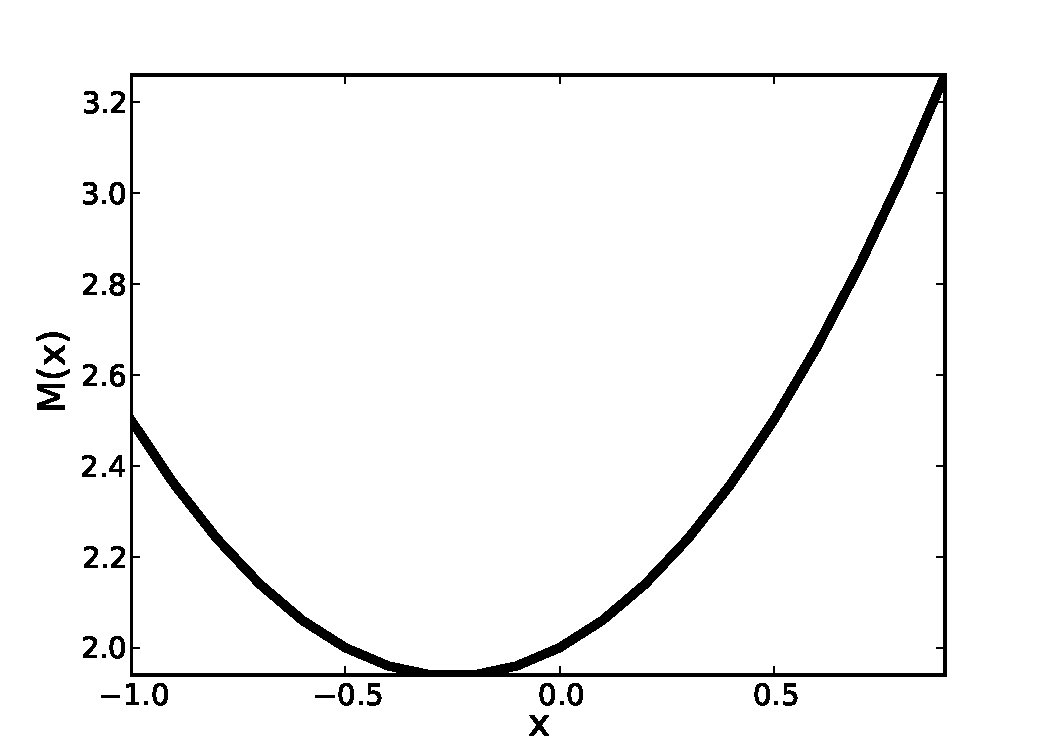
\epsfig{file=figs/mean.pdf,width=8cm}
    \caption{The mean function generated by \code{pymc/examples/gp/mean.py}.}
    \label{fig:mean}
\end{figure}

The mean function of a univariate GP is a unary function that can be interpreted as a prior guess for the GP. Mean functions are represented by \code{Mean} objects, which are wrappers for ordinary \proglang{Python} functions. The following code (from \code{pymc/examples/gp/mean.py}) will produce an instance of class \code{Mean} called $M$:
\begin{CodeChunk}
\begin{CodeInput}
from pymc.gp import *
def quadfun(x, a, b, c):
    return (a * x ** 2 + b * x + c)
M = Mean(quadfun, a = 1., b = .5, c = 2.)        
\end{CodeInput}
\end{CodeChunk}

The first argument of \code{Mean}'s init method is the underlying \proglang{Python} function, in this case \code{quadfun}. The extra arguments $a$, $b$  and $c$ will be memorized and passed to \code{quadfun} whenever $M$ is called; the call $M(x)$ in the plotting portion of \code{pymc/examples/gp/Mean.py}, which produces Figure~\ref{fig:mean}, does not need to pass them in.

Mean functions broadcast over their arguments in the same way as \pkg{NumPy} universal functions \citep{numpybook}, which means that the call $M(x)$, where $x$ is a vector, returns the vector
\begin{eqnarray*}
    [M(x_0),\ldots, M(x_{N_x-1})].
\end{eqnarray*}

The last part of the code plots $M(x)$ on $-1<x<1$, and its output is shown in Figure~\ref{fig:mean}. As expected, the plot is a parabola.

\subsection{Creating a covariance function}\label{subsub:cov}
\begin{figure}
    \centering
        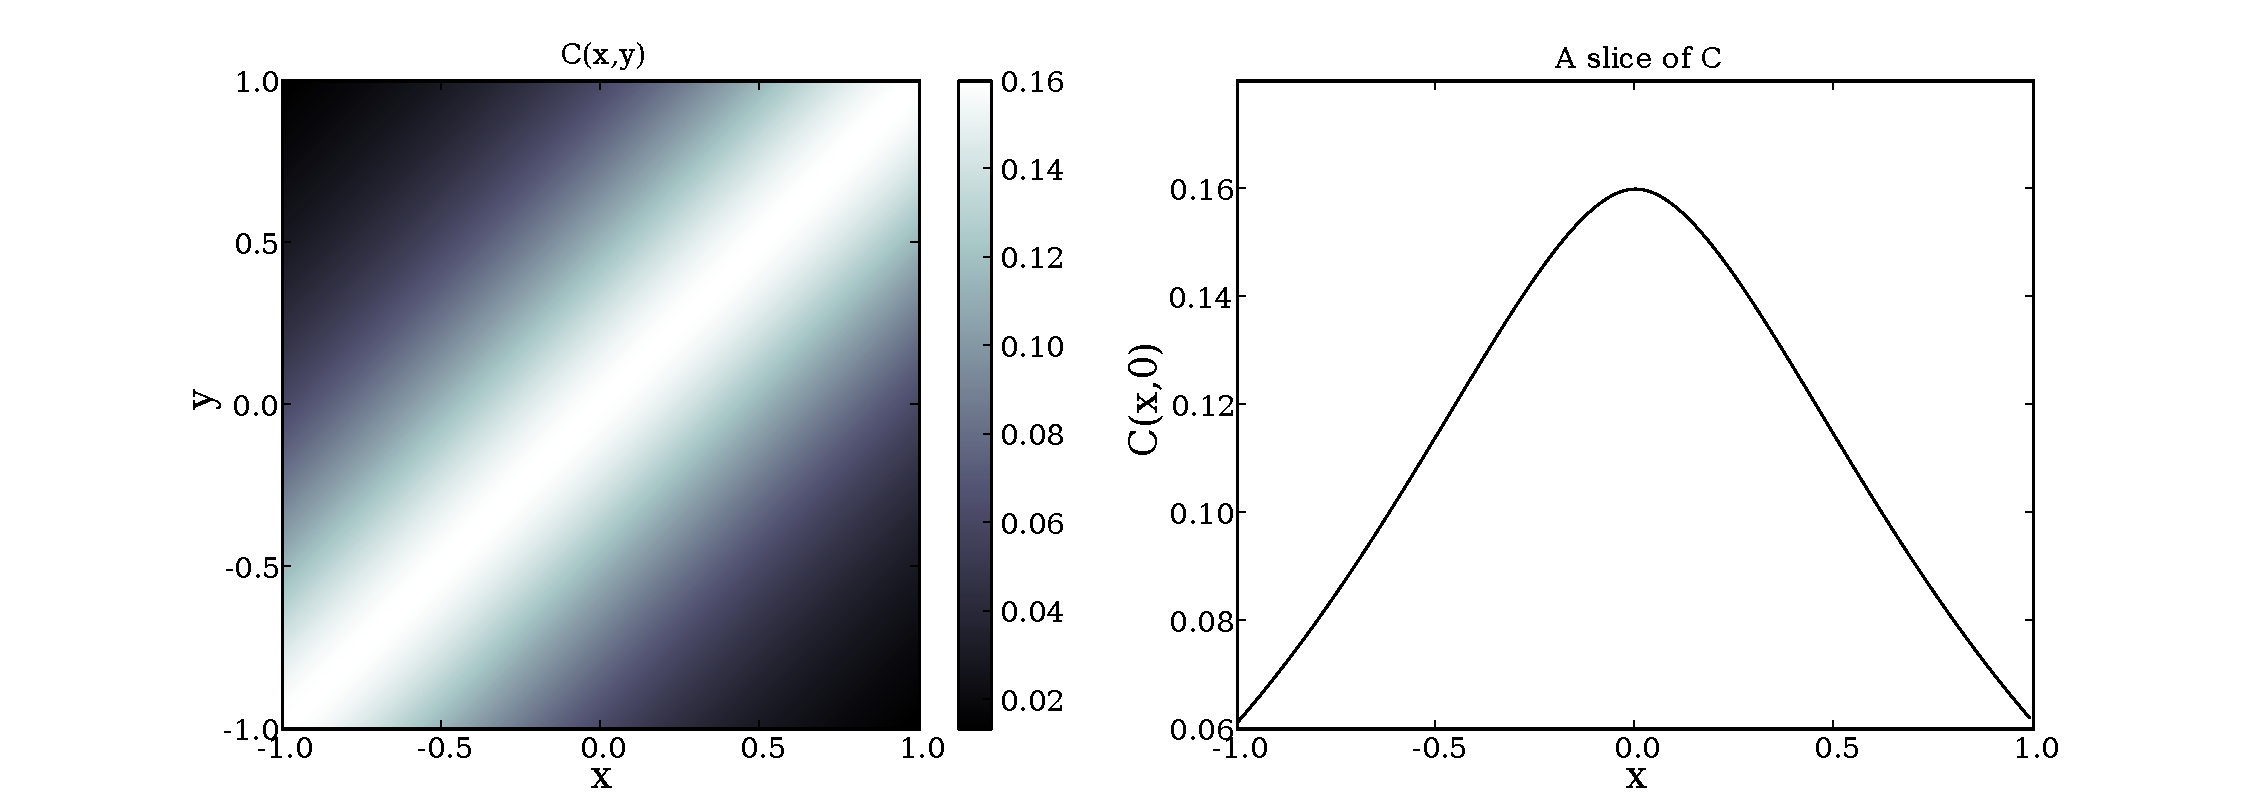
\epsfig{file=figs/cov.pdf,width=15cm}
    \caption{The covariance function generated by \code{pymc/examples/gp/cov.py}. On the left is the covariance function $C(x,y)$ evaluated over a square: $-1\le x\le 1,\ -1\le y\le 1$. On the right is a slice of the covariance: $C(x,0)$ for $0\le x \le 1$}
    \label{fig:cov}
\end{figure}

Covariance functions are represented by the class \code{Covariance}, which like \code{Mean} is essentially a wrapper for ordinary \proglang{Python} functions. The example in \code{pymc/examples/gp/cov.py} uses the popular Mat\`ern function \citep{banerjee}, which is provided in module \code{cov_funs}. In addition to the two arguments $x$ and $y$, the Mat\`ern function takes three parameters: \code{amp} controls the amount by which realizations may deviate from their mean, \code{diff_degree} controls the roughness of realizations (the degree of differentiability), and \code{scale} controls the lengthscale over which realizations change.

The user is free to write functions to wrap in \code{Covariance} objects. See the full package documentation at \href{http://pymc.googlecode.com/files/GPUserGuide.pdf}{http://pymc.googlecode.com/files/GPUserGuide.pdf} for more information.

The code in \code{pymc/examples/gp/cov.py} will produce an instance of class \code{Covariance} called $C$:
\begin{CodeChunk}
\begin{CodeInput}
from pymc.gp import *
from pymc.gp.cov_funs import matern

C = Covariance(eval_fun = matern.euclidean, diff_degree = 1.4, amp = .4, scale = 1.)
\end{CodeInput}
\end{CodeChunk}

The first argument to \code{Covariance}'s init method is the \proglang{Python} function from which the covariance function will be made. In this case, \code{eval_fun} is \code{matern.euclidean}. Covariance functions' calling conventions are slightly different from ordinary \pkg{NumPy} universal functions' \citep{numpybook} in two ways. First, broadcasting works differently. If $C$ were a \pkg{NumPy} universal function, $C(x,y)$ would return the following array:
    \begin{eqnarray*}
        \begin{array}{ccc}
            [C(x_0,y_0)& \ldots& C(x_{N_x-1},y_{N_x-1})],
        \end{array}
    \end{eqnarray*}
    where $x$ and $y$ would need to be vectors of the same length $N_x$. In fact $C(x,y)$ returns a matrix:
    \begin{eqnarray*}
        \left[\begin{array}{ccc}
            C(x_0,y_0)& \ldots& C(x_0,y_{N_y-1})\\
            \vdots&\ddots&\vdots\\
            C(x_{N_x-1},y_0)& \ldots& C(x_{N_x-1},y_{N_y-1})
        \end{array}\right],
    \end{eqnarray*}
    and input arguments $x$ and $y$ can have different lengths $N_x$ and $N_y$. Second, covariance functions can be called with just one argument. $C(x)$ returns
    \begin{eqnarray*}
         [C(x_0,x_0)& \ldots& C(x_{N_x-1},x_{N_x-1})]
    \end{eqnarray*}
    but is computed much faster than diag$(C(x,x))$ would be.
The extra arguments \code{diff_degree, amp} and \code{scale}, which are required by \code{matern.euclidean}, will be passed to \code{matern.euclidean} by $C$ every time it is called.
 
The output of \code{pymc/examples/gp/cov.py} is shown in Figure~\ref{fig:cov}.

\subsubsection{Cholesky algorithms}

The numerical `heavy lifting' required by this package is mostly done by \code{Covariance} and its subclasses. \code{Covariance} itself bases all its computations on the incomplete Cholesky decomposition algorithm used by the \proglang{Matlab} package \pkg{chol_incomplete} \citep{seeger}. \code{Covariance} computes rows of covariance matrices as they are needed, so if the function it wraps tends to produce covariance matrices with only a few large eigenvalues it can approximate the Cholesky decomposition in less than $O(n^2)$ arithmetic operations \citep{predictivechol}.

\code{Covariance} calls back to \proglang{Python} from \proglang{Fortran} every time it needs a new row. If the function it wraps tends to produce full-rank covariance matrices (for which all rows are required), this is inefficient. \code{FullRankCovariance} is a drop-in replacement for \code{Covariance} that is much faster, but fails (with a helpful error message) if it attempts to factor a matrix that is not of full rank. \code{NearlyFullRankCovariance} provides a compromise between the two: it computes covariance matrices in full in \proglang{Fortran}, then factors them using the robust algorithm of \pkg{chol_incomplete}.

\subsection{Drawing realizations}\label{subsub:realizations}
\begin{figure}
    \centering
        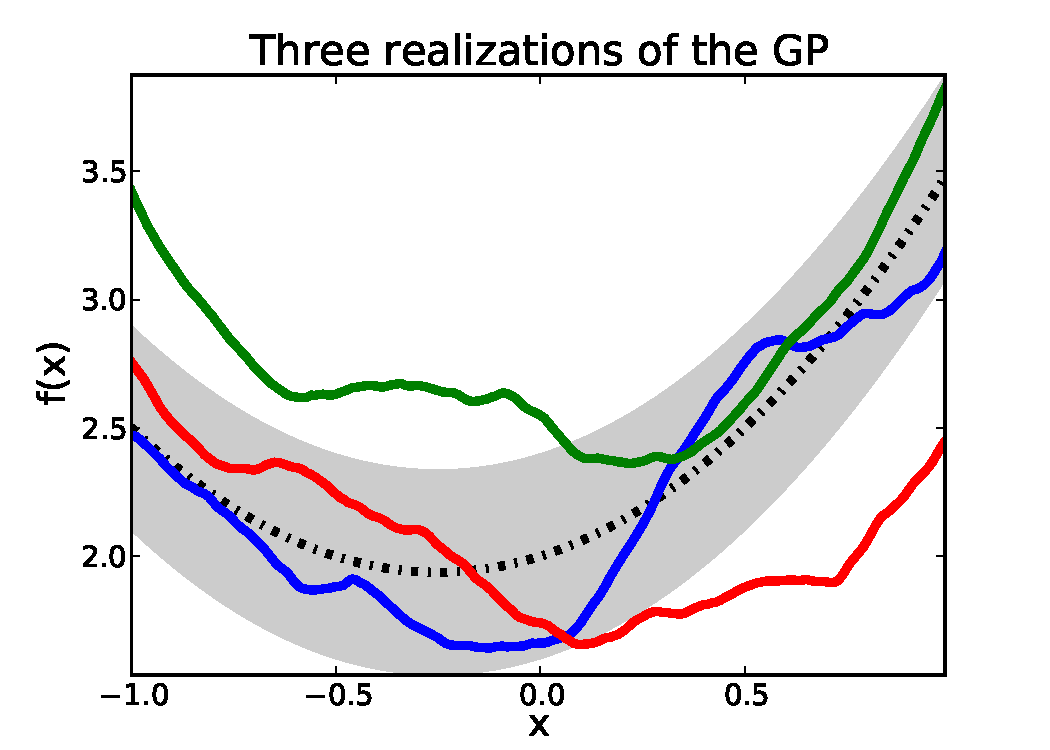
\epsfig{file=figs/realizations.pdf,width=10cm}
    \caption{Three realizations from a GP generated by \code{pymc/examples/gp/realizations.py} displayed with mean and a $\pm$ one standard deviation envelope.}
    \label{fig:realizations}
\end{figure}

The code in \code{pymc/examples/gp/realizations.py} generates a list of \code{Realization} objects, which represent realizations (draws) from the GP defined by $M$ and $C$:
\begin{CodeChunk}
\begin{CodeInput}
from mean import M
from cov import C
from pymc.gp import *

f_list = [Realization(M,C) for i in range(3)]
\end{CodeInput}
\end{CodeChunk}

The init method of \code{Realization} takes only two required arguments, a \code{Mean} object and a \code{Covariance} object. Each element of \code{f_list} is a GP realization, which is essentially a randomly-generated \proglang{Python} function. Like \code{Mean} objects, \code{Realization} objects use the same broadcasting rules as \pkg{NumPy} universal functions. The call $f(x)$ returns the vector
\begin{eqnarray*}
    [f(x_0)\ldots f(x_{N_x-1})].
\end{eqnarray*}

Each of the three realizations in \code{f_list} is plotted in Figure~\ref{fig:realizations}, superimposed on a $\pm$ 1 standard deviation envelope.


\section{Nonparametric regression: observing GPs}\label{sec:observing}

\begin{figure}
    \centering
        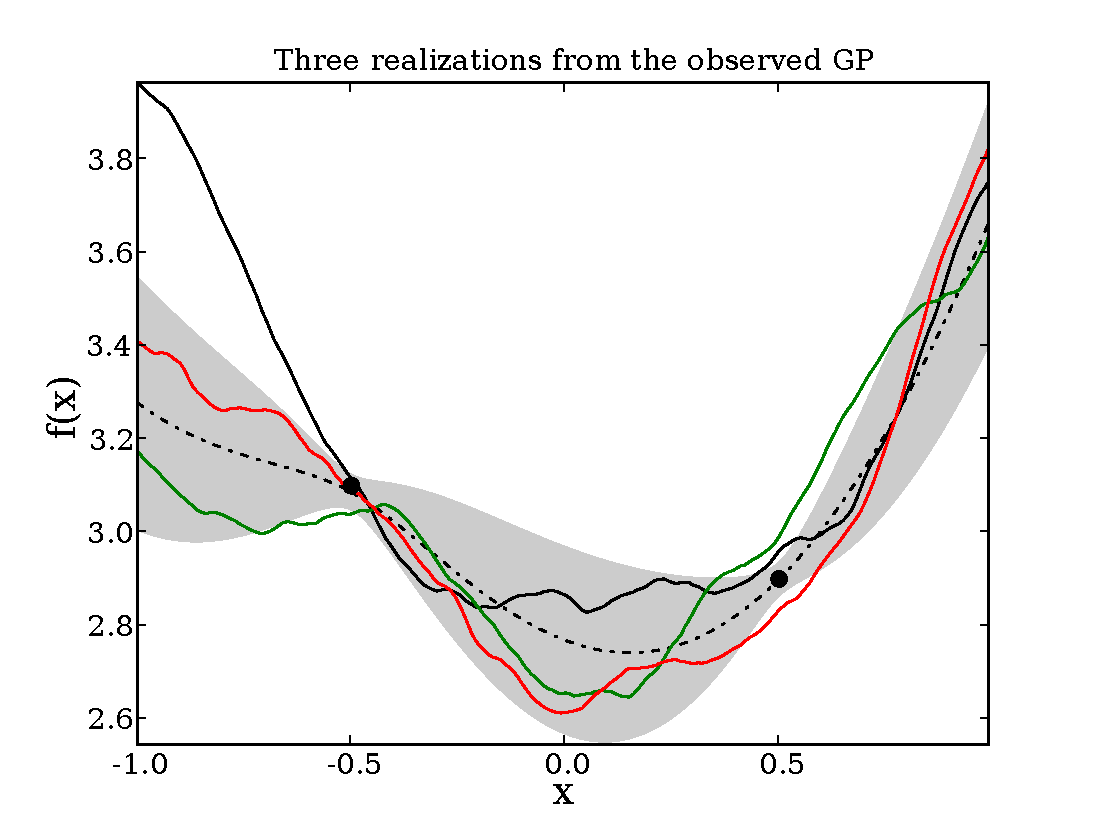
\epsfig{file=figs/obs.pdf,width=10cm}
        % 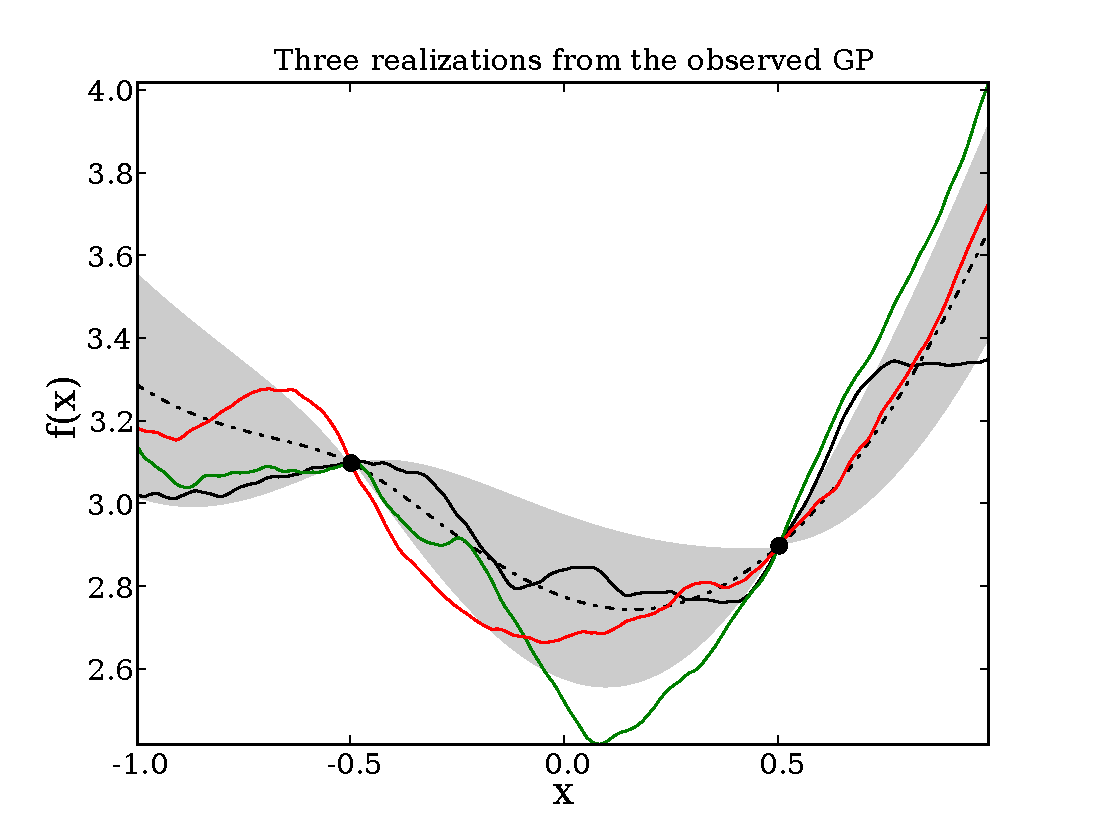
\epsfig{file=figs/cond.pdf,width=7cm}
    \caption{The output of \code{pymc/examples/gp/observations.py}. The uncertain observation of $f$'s value at $o=[-.5,.5]$ has been incorporated to produce a posterior distribution. The observed values are shown as black dots. Realizations from the posterior are more constrained at the observation points than realizations from the prior, shown in Figure~\ref{fig:realizations}.}
    \label{fig:obs}
\end{figure}

Consider the common statistical situation in which a GP prior for an unknown function $f$ is chosen with mean and covariance $M$ and $C$, and the value of $f$ is subsequently observed at $N_o$ input points $[o_0\ldots o_{N_o-1}]$, possibly with uncertainty. If the observation error is normally distributed, it turns out that $f$'s posterior distribution given the new information is another GP, with new mean and covariance functions $M_o$ and $C_o$ given by:
\begin{equation}
    \label{eq:obs-formula}
    blah 
\end{equation}

The probability model that represents this situation is as follows:
\begin{equation}
    \label{regprior}
    \left.\begin{array}{l}
        \textup{data}_i \stackrel{\tiny{\textup{ind}}}{\sim} \textup{N}(f(o_i), V_i)\\
        f \sim \textup{GP}(M,C)\\
    \end{array}\right\}\Rightarrow f|\textup{data} \sim \textup{GP}(M_o, C_o).
\end{equation}
Function \code{observe} imposes normally-distributed observations on GP distributions. This function converts $f$'s prior to its posterior by transforming $M$ and $C$ in equation~\ref{regprior} to $M_o$ and $C_o$.

The code in \code{pymc/examples/gp/observation.py} imposes the observations
\begin{eqnarray*}
    f(-.5) = 3.1\\
    f(.5) = 2.9
\end{eqnarray*}
with observation variance $V=.002$ on the GP defined in \code{mean.py} and \code{cov.py}:
\begin{CodeChunk}
\begin{CodeInput}
from mean import M
from cov import C
from pymc.gp import *
from numpy import *

o = array([-.5,.5])
V = array([.002,.002])
data = array([3.1, 2.9])
observe(M, C, obs_mesh=o, obs_V=V, obs_vals=data)

f_list = [Realization(M,C) for i in range(3)]
\end{CodeInput}
\end{CodeChunk}

The function \code{observe} takes a covariance $C$ and a mean $M$ as arguments, and tells them that their `true' realization's value on \code{obs_mesh} has been observed to be \code{obs_vals} with variance \code{obs_V}. 

The output of \code{observation.py}  is shown in figure \ref{fig:obs}, along with the output with \code{obs_V=0}. Compare these to the analogous figure for the unobserved GP, figure \ref{fig:realizations}. The covariance after observation is visualized in figure \ref{fig:obscov}. The covariance `tent' has been pressed down at points where $x\approx \pm .5$ and/or $y\approx\pm .5$, which are the values where the observations were made.

\begin{figure}
    \centering
        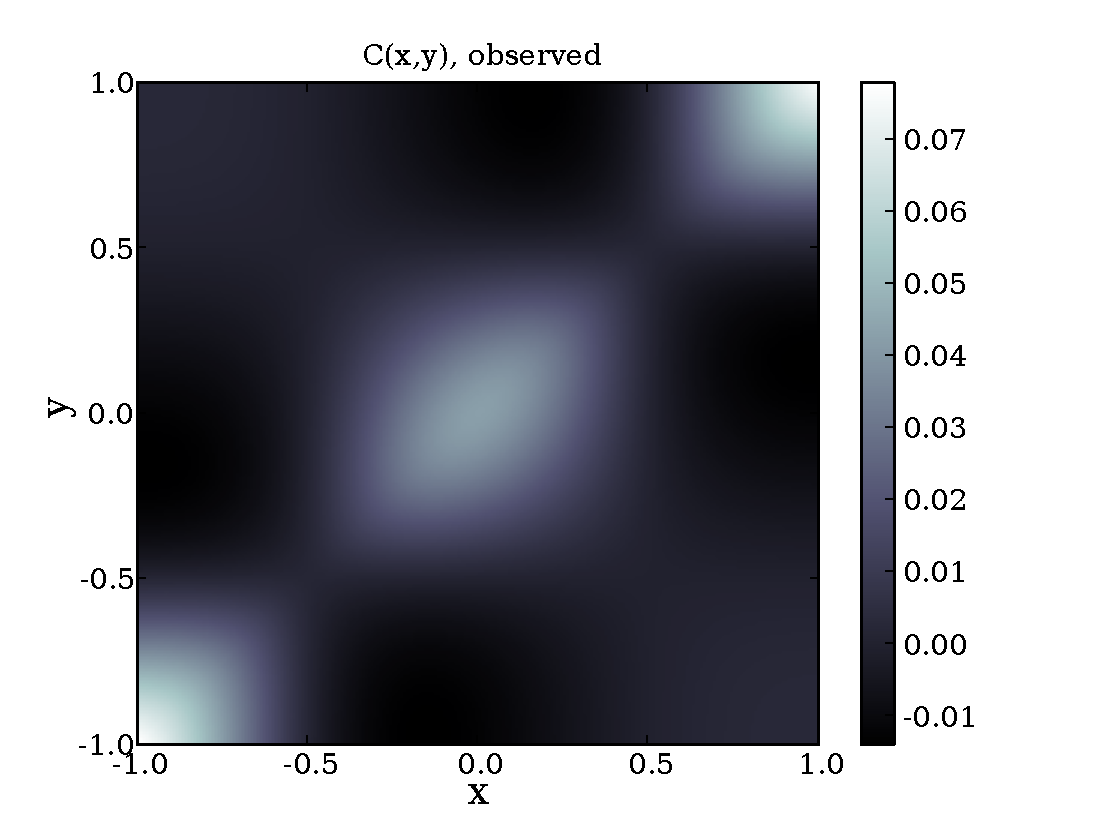
\epsfig{file=figs/obscov.pdf,width=5cm}
    \caption{The covariance function from {\sffamily `observation.py'} after observation. Compare this with the covariance function before observation, visualized in figure \ref{fig:cov} }
    \label{fig:obscov}
\end{figure}

\section{Higher-dimensional GPs}\label{sec:highdim}

In addition to functions of one variable such as $f(x)$, this package supports GP priors for functions of many variables such as $f(\mathbf{x})$, where $\mathbf{x}=[x_0\ldots x_{n-1}]$. Multivariate GPs are useful for modeling dynamical or biological functions of many variables as well as for spatial statistics.

When an array is passed into a \code{Mean}, \code{Covariance} or \code{Realization}'s init method or one of these objects is evaluated on an array, the array's last index is understood to iterate over spatial dimension. To evaluate a covariance $C$ on the ordered pairs $(0,1)$, $(2,3)$, $(4,5)$ and $(6,7)$, the user could pass in the following two-dimensional \pkg{NumPy} array:
\begin{verbatim}
[[0,1]
 [2,3]
 [4,5]
 [6,7]]
\end{verbatim}
or the following three-dimensional array:
\begin{verbatim}
[[[0,1]
  [2,3]],

  [4,5]
  [6,7]]]
\end{verbatim}
In both arrays, the last index is understood to iterate over elements of ordered pairs.

The exception to this rule is one-dimensional input arrays. The array
\begin{verbatim}
[0, 1, 2, 3, 4, 5, 6, 7]
\end{verbatim}
is interpreted as an array of eight one-dimensional values, whereas the array
\begin{verbatim}
[[0, 1, 2, 3, 4, 5, 6, 7]]
\end{verbatim}
is interpreted as a single eight-dimensional value according to the convention above.

Means and covariances learn their spatial dimension the first time they are called or observed. Some covariances, such as those specified in geographic coordinates, have an intrinsic spatial dimension. Realizations inherit their spatial dimension from their means and covariances when possible, otherwise they infer it the first time they are called. If one of these objects is subsequently called with an input of a different dimension, it raises an error.

\subsection{Covariance function bundles and coordinate systems}
The examples so far, starting with \code{pymc/examples/gp/cov.py}, have used the covariance function \code{matern.euclidean}. This function is an attribute of the \code{matern} object, which is an instance of class \code{covariance_function_bundle}.

Instances of \code{covariance_function_bundle} have three attributes, \code{euclidean}, \code{geo_deg} and \code{geo_rad}, which correspond to standard coordinate systems:
\begin{itemize}
    \item \code{euclidean}: $n$-dimensional Euclidean coordinates.
    \item \code{geo_deg}: Geographic coordinates (longitude, latitude) in degrees, with unit radius.
    \item \code{geo_rad}: Geographic coordinates (longitude, latitude) in radians, with unit radius.
\end{itemize}

See the full package documentation at \href{http://pymc.googlecode.com/files/GPUserGuide.pdf}{http://pymc.googlecode.com/files/GPUserGuide.pdf} for information regarding creation and extension of covariance function bundles.

\section{Basis covariances}\label{sec:basis}

\begin{figure}[htbp]
    \centering
        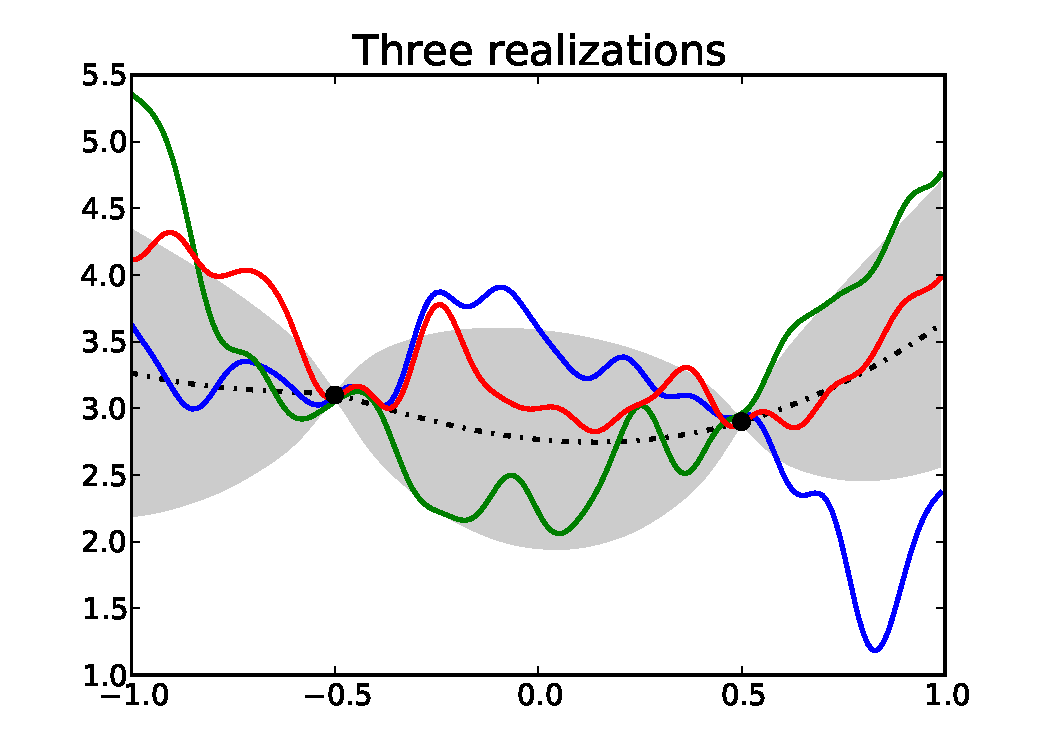
\epsfig{file=figs/basiscov.pdf,width=10cm}
        \caption{The output of \code{pymc/examples/gp/basis_cov.py} shows three realizations of an observed GP whose covariance is an instance of \code{BasisCovariance}. The basis in this case is function \code{fourier_basis} from module \code{cov_funs}. 25 basis functions are used. The realizations are substantially smoother than those in Figure~\ref{fig:obs}.}
    \label{fig:basiscov}
\end{figure}

It is possible to create GP's from linear combinations of finite sets of basis functions $\{e\}$ with random coefficients $\{c\}$. This approach can be computationally advantageous if the number of observation locations is large, and if the modeller has reason to believe that $f$ is infinitely differentiable or otherwise constrained. This package provides the \code{BasisCovariance} class to make it possible to take advantage of this optimization without requiring changes in user code. 

If $f$ is constructed as follows:
\begin{equation}
    \label{eq:basis-construction} 
    \begin{array}{l}
        f(x) = M(x) + \sum_{i_0=0}^{n_0-1}\ldots \sum_{i_{N-1}=0}^{n_{N-1}-1} c_{i_1\ldots i_{N-1}} e_{i_1\ldots i_{N-1}}(x), \\
        \{c\}\sim \textup{N}(0,K),
    \end{array}
\end{equation}
it follows that $f$ is a GP with mean $M$ and covariance defined by
\begin{eqnarray*}
    C(x,y)=\sum_{i_0=0}^{n_0-1}\ldots \sum_{i_{N-1}=0}^{n_{N-1}-1} \sum_{j_0=0}^{n_0-1}\ldots \sum_{j_{N-1}=0}^{n_{N-1}-1} e_{i_0\ldots i_{N-1}}(x) e_{j_0\ldots j_{N-1}}(x) K_{i_0\ldots i_{N-1}, j_0\ldots j_{N-1}},
\end{eqnarray*}
where $K$ is the covariance of the coefficients $c$.

Particularly successful applications of this general idea are random Fourier series, for which $e_i(x) = \sin(i\pi x/L)$ or $\cos(i\pi x/L)$ \citep{spanos}, and GP convolutions, for which $e_i(x) = \exp(-(x-\mu_n)^2)$ (or another kernel function) \citep{convolution}. Such representations can be very efficient when there are many observations in a low-dimensional space, but they are relatively inflexible in that they generally produce realizations that are infinitely differentiable. In some applications, this tradeoff makes sense.

This package supports basis representations via the \code{BasisCovariance} class:
\begin{verbatim}
    C = BasisCovariance(basis, cov, **basis_params)
\end{verbatim}
The arguments are:
\begin{description}
    \item[\code{basis}:] An array of functions, of any shape. Each basis function will be evaluated at $x$ with the extra parameters. The basis functions should obey the same calling conventions as mean functions: return values should have shape \code{x.shape[:-1]} unless $x$ is one-dimensional, in which case return values should be of the same shape as \code{x}. Note that each function should take the entire input array as an argument.
    \item[\code{cov}:] An array whose shape is either:
        \begin{itemize}
            \item Of the same shape as \code{basis}. In this case the coefficients are assumed independent, and \code{cov[i[0],...,i[N-1]]} (an $N$-dimensional index) simply gives the prior variance of the corresponding coefficient.
            \item Of shape \code{basis.shape * 2}, using \proglang{Python}'s convention for tuple multiplication. In this case \code{cov[i[0],...,i[N-1], j[0],...,j[N-1]]} (a $2N$-dimensional index) gives the covariance of $c_{i_0\ldots i_{N-1}}$ and $c_{j_1\ldots j_{N-1}}$.
        \end{itemize}
        Internally, the basis array is ravelled and the covariance tensor is reshaped into a matrix. This input convention makes it easier to keep track of which covariance value corresponds to which coefficients. The covariance tensor must be symmetric (\code{cov[i[0],...,i[N-1], j[0],...,j[N-1]]} $=$ \code{cov[j[0],...,j[N-1], i[0],...,i[N-1]]}), and positive semidefinite when reshaped to a matrix.
    \item[\code{basis_params}:] Any extra parameters required by the basis functions.
\end{description}

\section{Separable bases}

Many bases, such as Fourier series, can be decomposed into products of functions as follows:
\begin{eqnarray*}
    e_{i_0\ldots i_{N-1}}(x) = \prod_{j=0}^{N-1}e_{i_j}^j(x)
\end{eqnarray*}
Basis covariances constructed using such bases can be represented more efficiently using \code{SeparableBasisCovariance} objects. These objects are constructed just like \code{BasisCovariance} objects, but instead of an $n_0\times \ldots \times n_{N-1}$ array of basis functions they take a nested lists of functions as follows:
\begin{verbatim}
    basis = [ [e[0][0], ... ,e[0][n[0]-1]]
                       ...
              [e[N-1][0], ... ,e[N-1][n[N-1]-1]] ].
\end{verbatim}
For an $N$-dimensional Fourier basis, each of the \code{e}'s would be a sine or cosine; frequency would increase with the second index. As with \code{BasisCovariance}, each basis needs to take the entire input array \code{x} and \code{basis_params} as arguments. See \code{fourier_basis} in \code{pymc/examples/gp/basiscov.py} for an example.

\subsection{Example}

Once created, a \code{BasisCovariance} or \code{SeparableBasisCovariance} object behaves just like a \code{Covariance} object, but it and any \code{Mean} and \code{Realization} objects associated with it will take advantage of the efficient basis representation in their internal computations. An example of \code{SeparableBasisCovariance} usage is given in \code{pymc/examples/gp/basis_cov.py}. 

Its output, shown in Figure~\ref{fig:basiscov}, is analogous to Figure~\ref{fig:obs}. Unlike realizations generated using the Mat\`ern covariance, realizations generated using the basis covariance are infinitely differentiable (very smooth) because $f$ is constructed as a linear combination of a finite set of infinitely differentiable functions (equation~\ref{eq:basis-construction}). If $f$ is known a priori to be infinitely differentiable, this smoothness is not a problem; but if $f$ is believed to be more rough, as is often the case in geostatistics, basis covariances are not appropriate.


\section{Using Gaussian processes in Bayesian probability models}
\label{sec:gp-sub} 

Like any other random variable, a GP can be incorporated in a Bayesian probability model and its value can, at least conceptually, be inferred from data. Equation~\ref{regprior} provides a simple example: unknown function $f$ is assigned a GP prior, and the dependence of the data on it is modeled as follows:
\begin{eqnarray*}
    \textup{data}_i \stackrel{\tiny{\textup{ind}}}{\sim} \textup{N}(f(o_i), V_i)
    f \sim \textup{GP}(M,C).
\end{eqnarray*}
For this particular model, the posterior of $f$ is also a GP, and closed formulas for its mean and covariance can be produced.

For more general models, the posterior of $f$ is usually not of a standard form. As a concrete example, this section and the next will consider the nonparametric regression model implemented in \code{pymc/examples/gp/PyMCmodel.py}, which is a simple hierarchical extension of the model above. In the hierarchical model, the mean $M_{a,b,c}$ is a parabola with unknown coefficients $a$, $b$ and $c$. The covariance $C_{\nu,\theta,\phi}$ of $f$ is the Mat\`ern covariance with unknown degree of differentiability parameter $\nu$, lengthscale $\theta$, and amplitude $\phi^2$ so that $\mathsf{V}(f(x))=\phi^2$. The data $d$ are noisy measurements of $f$, with unknown measurement variance $V$, at unknown observation locations $o$. The full model specification, including priors for the scalar parameters, is
\begin{equation}
    \label{eq:simple-example-model} 
    \begin{array}{rr}
    \nu\sim\textup{Uniform}(1,3)&\\
    \phi\sim\textup{Lognormal}(.4,1)&\\
    \theta\sim\textup{Lognormal}(.5,1)&\\
    C_{\nu,\theta,\phi}(x,y) = \phi^2\textup{Mat\`ern}_\nu\left( \frac{x-y}{\theta} \right)&\\
    &\\
    a\sim\textup{Normal}(1,1)&\\
    b\sim\textup{Normal}(.5,1)&\\
    c\sim\textup{Normal}(2,1)&\\
    M_{a,b,c}(x) = ax^2+bx+c&\\
    &\\
    f|a,b,c,\nu,\theta,\phi\sim\textup{GP}(M_{a,b,c}, C_{\nu,\theta,\phi})&\\
    &\\
    V\sim\textup{Lognormal}(-1,1)&\\
    o_i \stackrel{\textup{\tiny ind}}{\sim} \textup{Normal}\left(-\frac{4}{5}+\frac{8}{15}(i-1), .0001\right),&i=1\ldots 4\\
    d_i|f,o_i,V \stackrel{\textup{\tiny ind}}{\sim} \textup{Normal}(f(o_i),V),& i=1\ldots 4
        \end{array}
\end{equation}
For this model, the posterior of $f$ does not have a standard form. In Bayesian analysis, nonstandard posteriors are commonly sampled using MCMC methods, but development of such methods for models like model \ref{eq:simple-example-model} is complicated by the fact that unknown functions on infinite domains (such as $\mathbb R$) are infinite-dimensional random variables. 

This package provides Metropolis-Hastings algorithms (see section~\ref{sec:step-methods}) that can be used by \pkg{PyMC} \citep{pymc} to sample the posteriors of Bayesian probability models involving GPs. The result produced by such algorithms for the model above (see section~\ref{sub:BasicMCMC}) is a sequence of approximate samples from the joint posterior of the unknown variables $a$, $b$, $c$, $\nu$, $\phi$, $\theta$ and $f$. Such sequences are also known as  `dynamic traces' \citep{gamerman}. 

\subsection{Splitting approach} 
\pkg{PyMC} represents random variables, such as $a$, $b$, $c$, $\nu$, $\phi$, $\theta$ and $f$, as objects of class \code{Stochastic}. For example, the following code produces the normally-distributed random variable $a$ in the model above:
\begin{CodeChunk}
\begin{CodeInput}
a = pymc.Normal('a',1,1)
\end{CodeInput}
\end{CodeChunk}
The current value of variable $a$ can be queried and updated as follows:
\begin{CodeChunk}
\begin{CodeInput}
print a.value
a.value = 0.5
\end{CodeInput}
\end{CodeChunk}
The logarithm of $a$'s prior probability density function, evaluated at its current value, can be obtained via \code{a.logp}. \pkg{PyMC} has a large library of optimized log-probability density/mass functions, and readily incorporates new functions created by users.

This package equips \pkg{PyMC} with GPs via \code{GaussianProcess} objects, which are random variables whose values are \code{Realization} objects. Because a GP is an infinite-dimensional variable, it is not practical to compute anything like a probability density for it, and \code{GaussianProcess}es have no \code{logp} attribute.

As discussed further in section \ref{sec:step-methods}, the lack of a probability density is problematic because Metropolis-Hastings acceptance ratios cannot be computed. However, given a finite vector $x_*$, the a GP $f$ can be split into two random variables:
\begin{eqnarray*}
    f\sim\textup{GP}(M,C) & \Leftrightarrow & \begin{array}{r}
        f(x_*)\sim\textup{Normal}(M(x_*), C(x_*,x_*))\\
        f|f(x_*)\sim\textup{GP}(M_{x_*}, C_{x_*})
    \end{array}
\end{eqnarray*}
where $M_{x_*}$ and $C_{x_*}$ are generated using equation \ref{eq:obs-formula} with $V=0$ and $d=f(x_*)$. This splitting does not change the marginal distribution of $f$, and therefore does not alter any model in which $f$ is embedded. Note that this is true regardless of $x_*$; $x_*$ does not have to coincide with the input locations.

The vector $f(x_*)$ is a simple multivariate normal random variable, which can be endowed with a \code{logp} attribute. For reasons explained in Section~\ref{sec:step-methods}, every \code{GaussianProcess} is wrapped in a \code{GPSubmodel} container object along with a multivariate normal variable representing its evaluation on a fixed, finite vector, called its `mesh'. As noted above, the mesh that is chosen does not affect the mathematical specification of the model (\emph{ie} the posterior), but can have a substantial effect on the performance of the MCMC algorithm (see section~\ref{sec:mesh-choice}).  

\subsection{Example: nonparametric regression with unknown mean and covariance parameters and unknown observation locations}\label{sub:BasicMCMC}

Model~\ref{eq:simple-example-model} is declared as a \pkg{PyMC} probability model in \code{examples/gp/PyMCModel.py}. Just as Bayesian probability models are linked collections of stochastic variables, \pkg{PyMC} probability models are linked collections of \code{Stochastic} variables. These variables may be scalar-valued like $a$, vector-valued like $f(x_*)$, or function-valued like $f$.

In \code{pymc/examples/gp/PyMCmodel.py}, a GP submodel that contains $f$ in model~\ref{eq:simple-example-model} is created as follows:
\begin{CodeChunk}
\begin{CodeInput}
sm = gp.GPSubmodel('sm',M,C,fmesh)
\end{CodeInput}
\end{CodeChunk}
The GP submodel contains two stochastic variables: \code{sm.f} and \code{sm.f_eval}. The first is the actual GP $f$, a stochastic variable valued as a \code{Realization} object. The second is $f(x_*)$, where $x_*$ is the constant vector \code{fmesh}.

Once the GP submodel has been created, other variables can depend on $f$ and $f(x_*)$ in any way that can be expressed in \proglang{Python} code. In the model above, the observation $d$ depends on $f(o)$, where $o$ are the observation locations. If $o$ were known in advance, $x_*$ could be chosen to be equal to $o$, so that $d$ depends on $f(x_*)$, and no other evaluations of $f$. As discussed in section \ref{sec:step-methods}, this parameterization is usually computationally advantageous (section~\ref{sec:mesh-choice}) and should be used when possible. 
\begin{CodeChunk}
\begin{CodeInput}
d = pymc.Normal('d',mu=sm.f_eval, tau=1./V, value=init_val, observed=True)
\end{CodeInput}
\end{CodeChunk}
In Section~\ref{sec:duffy}, a \code{GaussianProcess}'s children depend on it in a less standard way, and the observation locations are known a priori. 

The file \code{pymc/examples/gp/MCMC.py} fits the probability model specified in \code{\pkg{PyMC}model.py} using MCMC. The part of the file that actually dispatches the sampling loop is very simple:
\begin{CodeChunk}
\begin{CodeInput}
GPSampler = MCMC(PyMCmodel)
GPSampler.isample(iter=5000,burn=1000,thin=100)    
\end{CodeInput}
\end{CodeChunk}
The file's output is shown in Figure~\ref{fig:MCMCOutput}. After the MCMC loop has terminated, \\\code{GPSampler.trace('sm_f')[:]} yields a dynamic trace for \code{sm.f}. This is a sequence of \code{Realization} objects, which can be evaluated on new arrays for plotting. Traces for GP realizations can even be stored on disk via \pkg{PyTables} \citep{tables}, see \cite{pymc}.

% \begin{figure}
%     \centering
%         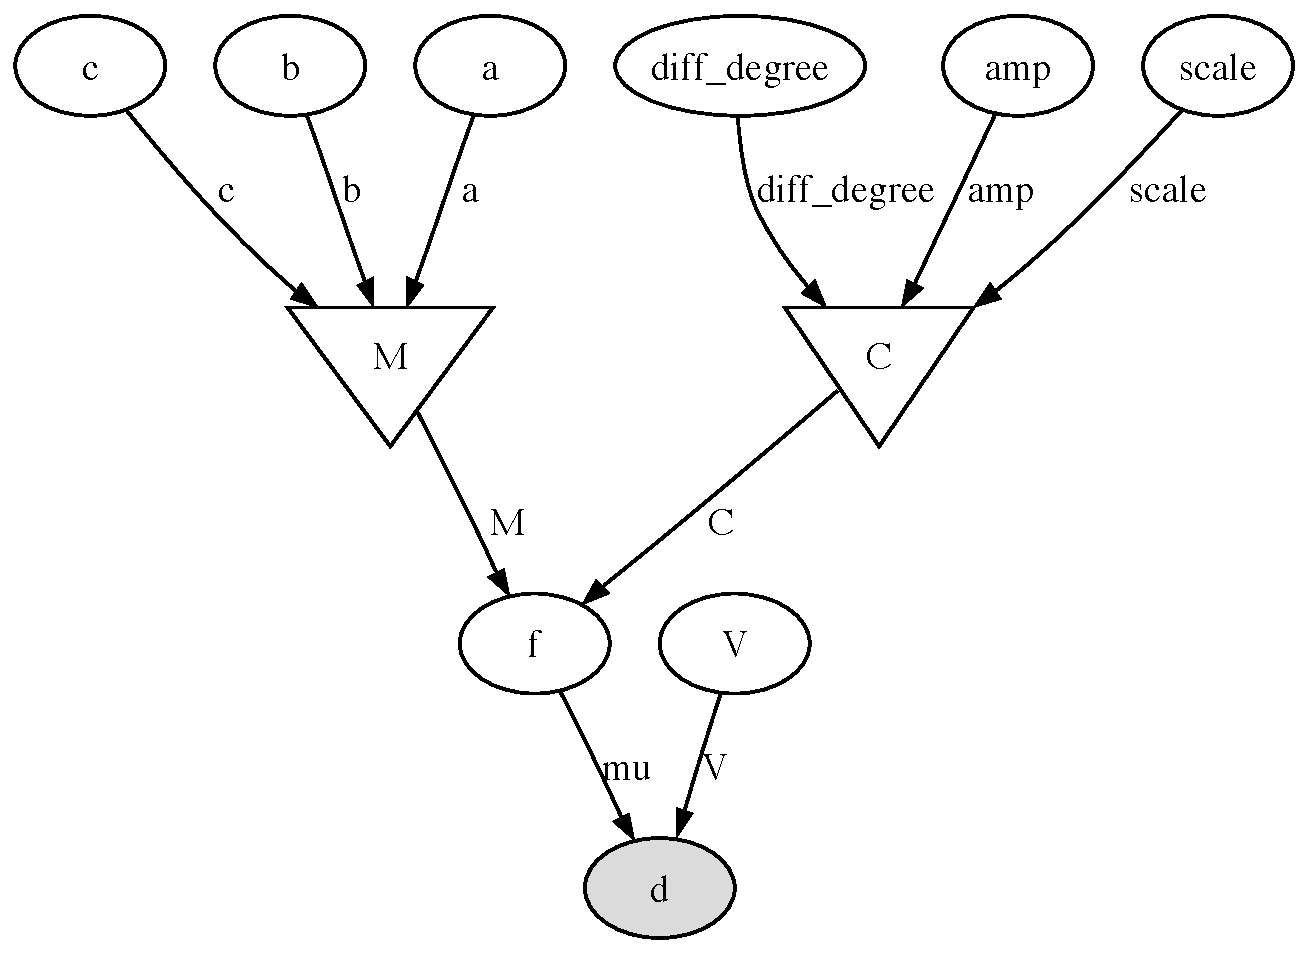
\epsfig{file=figs/unobservedModel.pdf, width=15cm}
%     \caption{The \pkg{PyMC}-generated directed acyclic graph representation of the extended nonparametric regression model created by \code{pymc/examples/gp/PyMCModel.py}. Ellipses represent \code{Stochastic} objects (variables whose values are unknown even if their parents' values are known), triangles represent \code{Deterministic} objects (variables whose values can be determined if their parents' values are known), and rectangles represent \code{Stochastic} objects with the \code{isdata} flag set to \code{True} (data). Rectangles represent potentials. Arrows point from parent to child. The submodel contains the GP \code{sm\_f} and its evaluation \code{sm\_f\_eval} on input array \code{sm\_mesh}. It also contains the mean \code{sm\_M\_eval} of \code{sm\_f\_eval} and the lower-triangular Cholesky factor \code{sm\_S\_eval} of its covariance matrix, and a potential \code{sm_fr_check} that forces that covariance matrix to remain positive definite. The actual covariance evaluation \code{sm\_C\_eval} is not needed by the model, but it is exposed for use by Gibbs step methods.}
%     \label{fig:unobservedModel}
% \end{figure}

\begin{figure}
    \centering
        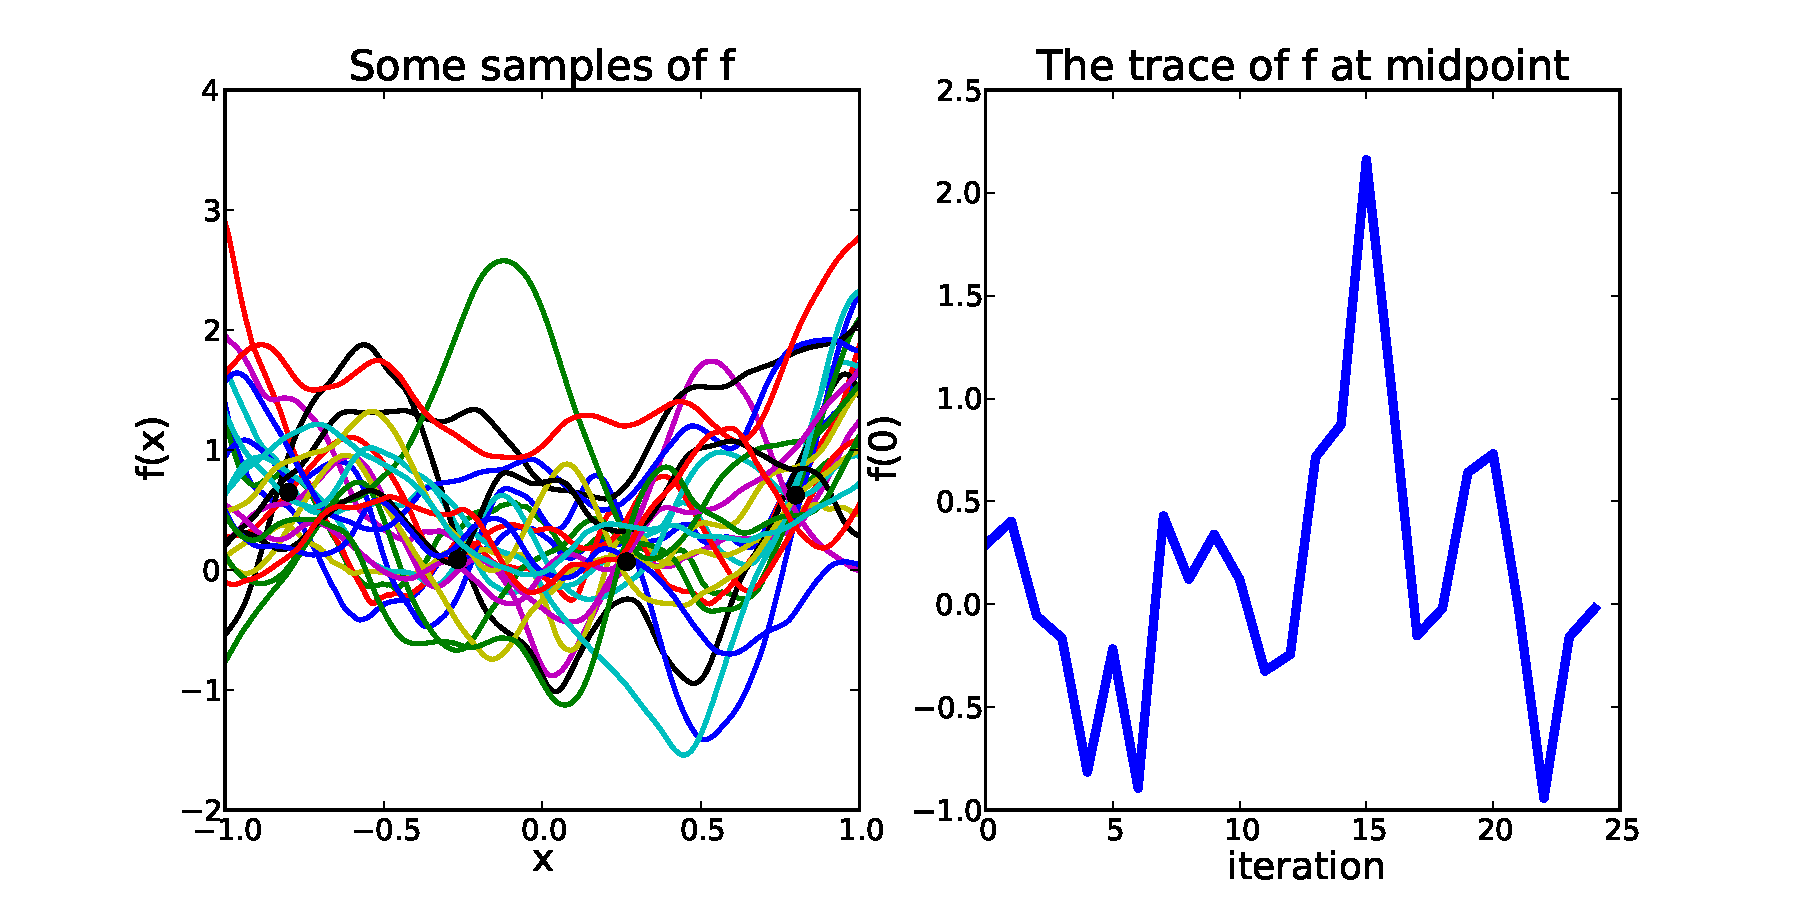
\epsfig{file=figs/gibbsSamples.pdf,width=10cm}
        % 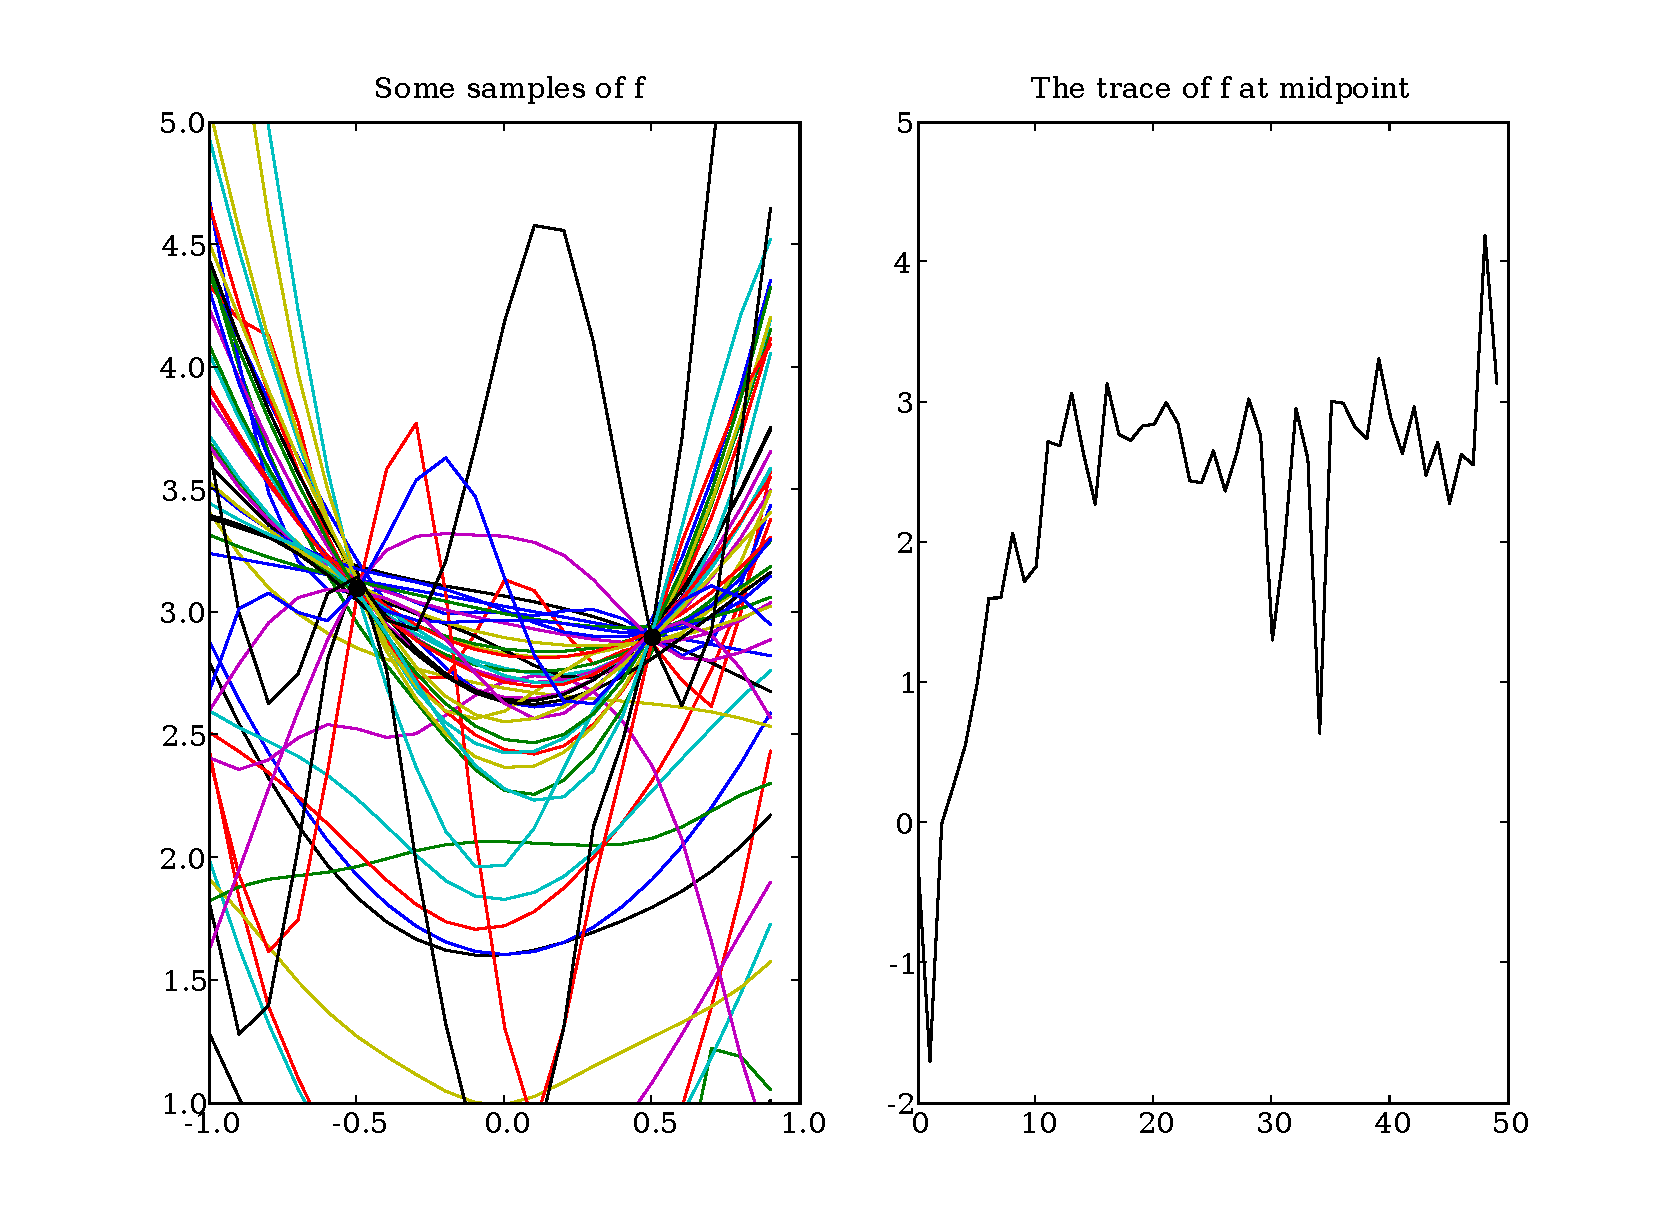
\epsfig{file=figs/metroSamples.pdf,width=10cm}
    \caption{The output of \code{pymc/examples/gp/MCMC.py}. The left-hand panel shows all the samples generated for the GP $f$, and the right-hand panel shows the trace of $f(0)$.}
    \label{fig:MCMCOutput}
\end{figure}
 

\section{Metropolis-Hastings algorithms for updating Gaussian processes}
\label{sec:step-methods}

\pkg{PyMC}'s core business is to produce approximate samples from the posteriors of probability models using the MCMC algorithm. Its implementation of the MCMC algorithm uses the usual modular strategy; in a single iteration, the value of each variable in the model is updated using a jumping rule whose stationary distribution is its full conditional distribution. A common jumping rule is the Metropolis-Hastings algorithm \citep{gamerman}. 

The implementation of each jumping rule is delegated to a \code{StepMethod} object. \citep{pymc}. Bespoke MCMC algorithms can be constructed by choosing which step methods to assign to each of the model's stochastic variables. The Metropolis-Hastings algorithm is implemented by the \code{Metropolis} step method. \code{Metropolis} and related step methods use on the \code{logp} attributes (see Section~\ref{sec:gp-sub}) of the variables they handle to compute acceptance ratios for proposed values. 

Recognizing that no single MCMC scheme can guarantee good performance for all probability models, \pkg{PyMC}'s overall approach to MCMC is to modularize the algorithm and make it easy for users to tune, alter or rewrite the jumping strategies it uses for individual variables. The Metropolis-Hastings algorithms provided by this package perform relatively well for the models of Bayesian geostatistics such as the example in section~\ref{sec:duffy}, but users may need to override them when working with more unusual model forms. In these cases, the Metropolis-Hastings scheme outlined in section~\ref{sec:step-methods} can still provide a useful starting point. The documentation and user community of \pkg{PyMC} are helpful resources for users who need to write their own jumping strategies. 



\subsection{Step methods that handle parents of Gaussian processes}
Because it is impractical to associate a probability density function with GPs, \code{GaussianProcess}es have no \code{logp} attribute and they cannot be handled by the Metropolis-Hastings family of step methods, because there is no way to calculate acceptance ratios. This package uses a relatively simple work-around that will be described in this section, a Metropolis-Hastings rule for updating the parents of GPs jointly with the GPs themselves. In the context of the model above, the GP itself is $f$ and the parents are $a$, $b$, $c$, $\nu$, $\phi$ and $\theta$. The parents of $f$ are denoted $P$ and the children $K$ throughout.

The updating rule is developed heuristically in this section by assuming the (false) premise that the probability density functions are available, then choosing the proposal distribution so as to avoid the need to evaluate them. The development can be made more rigorous by replacing $f$ with its evaluation at all the points at which its value would ever be needed.

Denote by $P$ the parents of a GP $f$ in an arbitrary probability model, perhaps the one in section \ref{sec:gp-sub}. Denote by $P_p$ and $f_p$ alternative `proposed' values for each. If a probability density function $p(f|P)$ for $f$, and a proposal density $q(f_p,P_p|f,p)$, were available, the Metropolis-Hastings acceptance ratio for jointly proposed values $P_p$ and $f_p$ would be:
\begin{eqnarray*}
    \frac{p(K|f_p)\ p(f_p|P_p)\ p(P_p)\ q(f,P|f_p,P_p)}{p(K|f)\ p(f|P)\ p(P)\ q(f_p,P_p|f,P)}.
\end{eqnarray*}
If the proposal is broken into two stages, so that a value $f_p$ is proposed conditional on proposed values for the parents $P_p$ \emph{and} $f_p(x_*)$, the acceptance ratio becomes
\begin{eqnarray*}
    \frac{p(K|f_p)\ p(f_p|f_p(x_*), P_p)\ p(f_p(x_*) | P_p)\ p(P_p)}{p(K|f)\ p(f|f(x_*), P)\ p(f(x_*) | P)\ p(P)}
    \frac{q(f|f(x_*),P,f_p)  }{q(f_p|f_p(x_*),P_p,f)}
    \frac{q(f(x_*),P|f_p,f_p(x_*),P_p)}{q(f_p(x_*),P_p|f,f(x_*), P)}
\end{eqnarray*}
Since, in practical terms, no density is available for the unknown functions $f$ and $f_p$, the terms with these variables in the consequent position cannot be evaluated:
\begin{equation}
    \label{eq:problem-terms} 
    \begin{array}{r}
        p(f_p|f_p(x_*), P_p),\\ q(f|f(x_*),P,f_p),\\ p(f|f(x_*), P),\\ q(f_p(x_*),P_p|f,f(x_*), P).
    \end{array}
\end{equation}
Fortunately, these can be made to cancel by choosing a proposal distribution as follows:
\begin{eqnarray*}
    q(f_p|f_p(x_*),P_p,f) = p(f_p|f_p(x_*), P_p).
\end{eqnarray*}
In other words, if $f$ is proposed from its prior distribution conditional on $f(x_*)$ and its parents whenever $f(x_*)$ is proposed, there is no need to compute the terms in expression~\ref{eq:problem-terms} .

\smallskip

To summarize, any Metropolis-Hastings step method can handle the parents of $f$ or $f(x_*)$, if it proposes values for $f$ jointly with its target variable as outlined above. This minor alteration in jumping strategy is implemented by the function \\\code{wrap_metropolis_for_gp_parents}, which takes a subclass of \code{Metropolis} as an argument and returns a new step method class with altered \code{propose} and \code{reject} methods. The function automatically produces modified versions of all Metropolis step methods implemented by \pkg{PyMC} \citep{pymc}. The modified step methods are automatically assigned to parents of GPs.

\subsection{Choosing a mesh} 
\label{sec:mesh-choice} 
The mesh points $x_*$ are the points where Metropolis-Hastings step methods can `grab' the value of $f$ to moderate the variance of its proposal distribution. If $x_*$ is an empty array, $f$'s value will be proposed from its prior, and rejection rates are likely to be quite large. If $x_*$ is too dense, on the other hand, computation of the log-probability of $f(x_*)$ will be expensive, as its cost scales as the cube of the number of points in the mesh. This continuum is illustrated in Figure~ \ref{fig:meshpropose}.

\begin{figure}
    \centering
        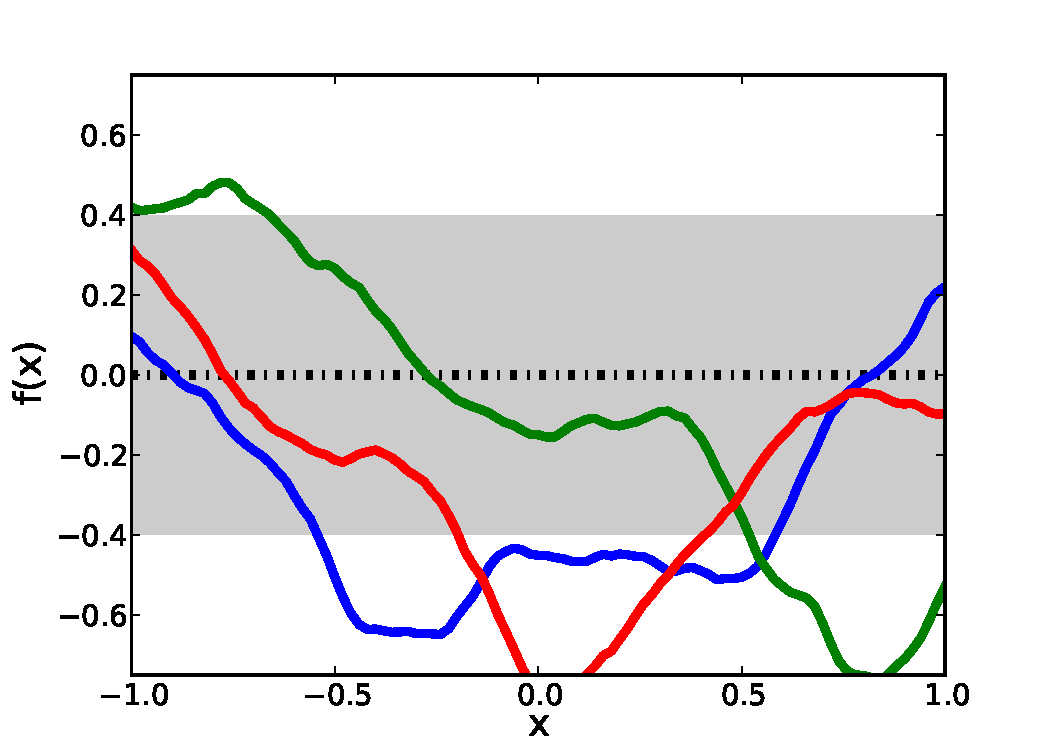
\epsfig{file=figs/nomeshpropose.pdf,width=5cm}
        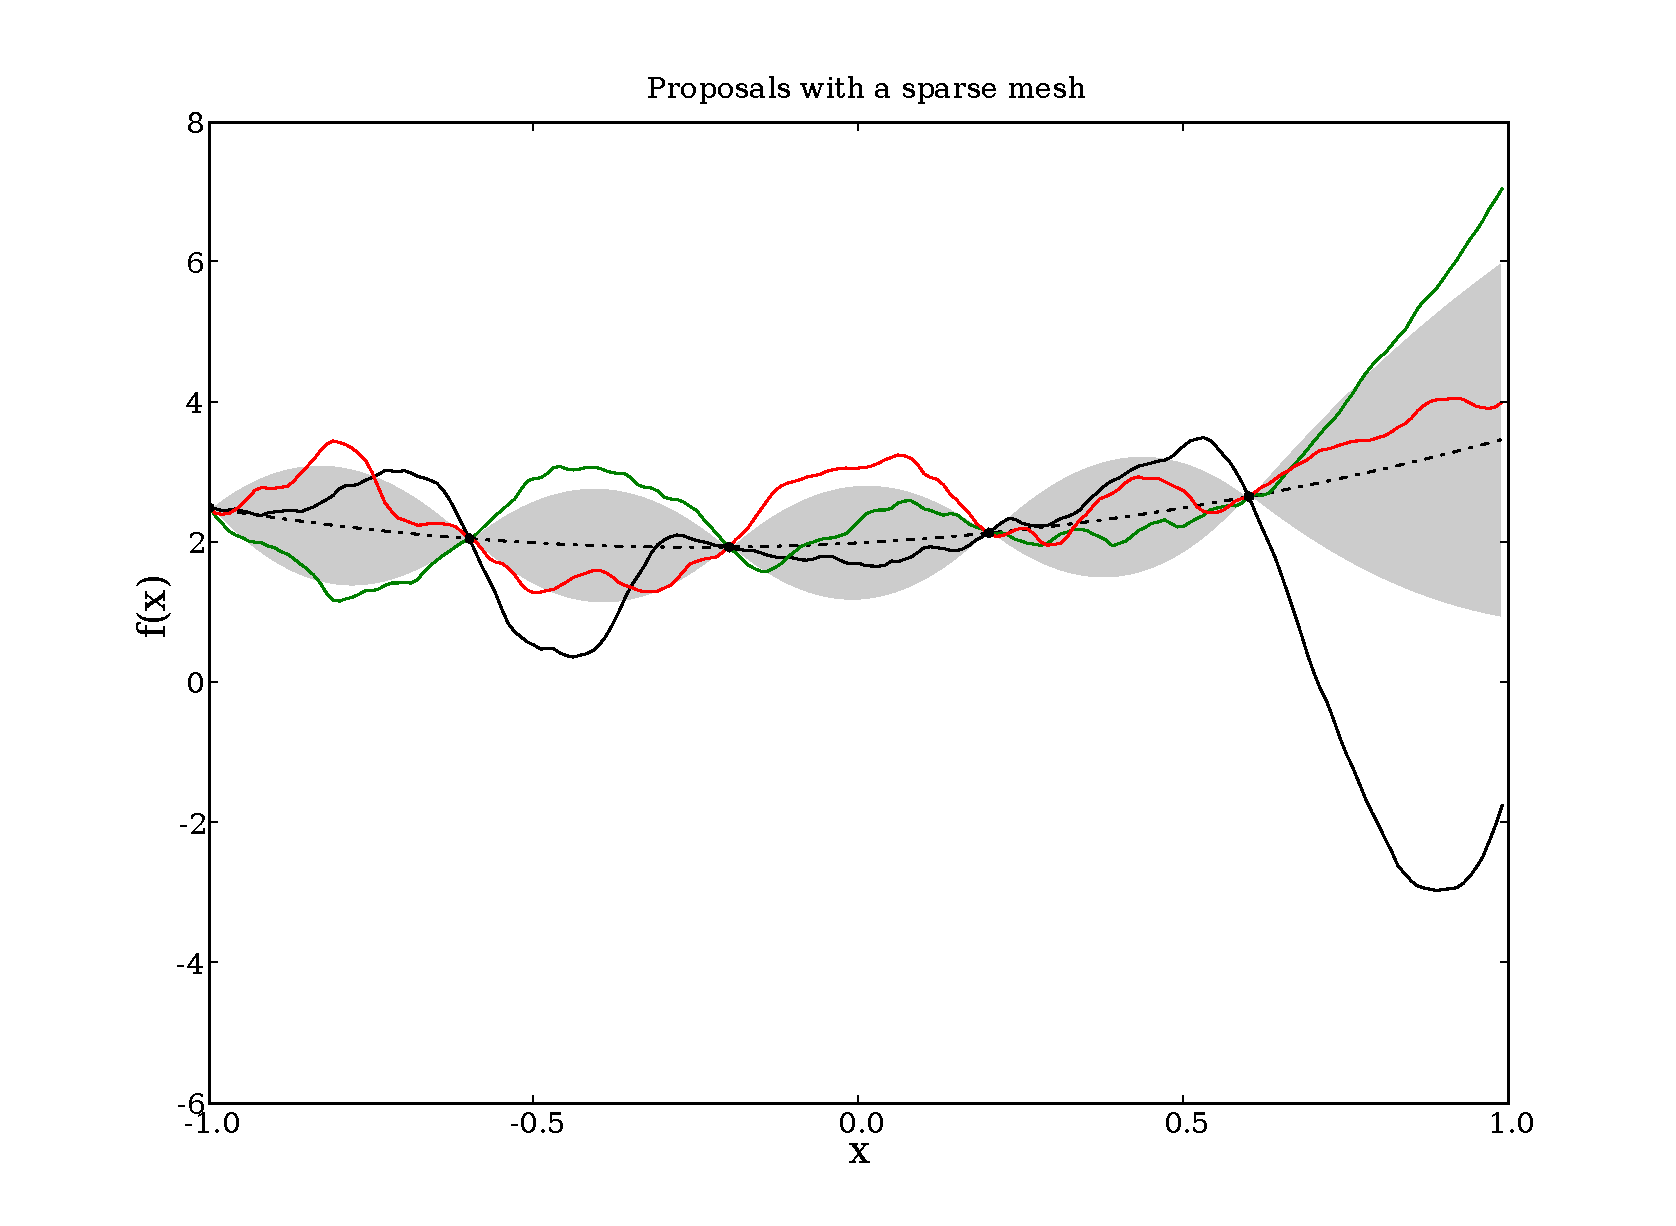
\epsfig{file=figs/lightmeshpropose.pdf,width=5cm}
        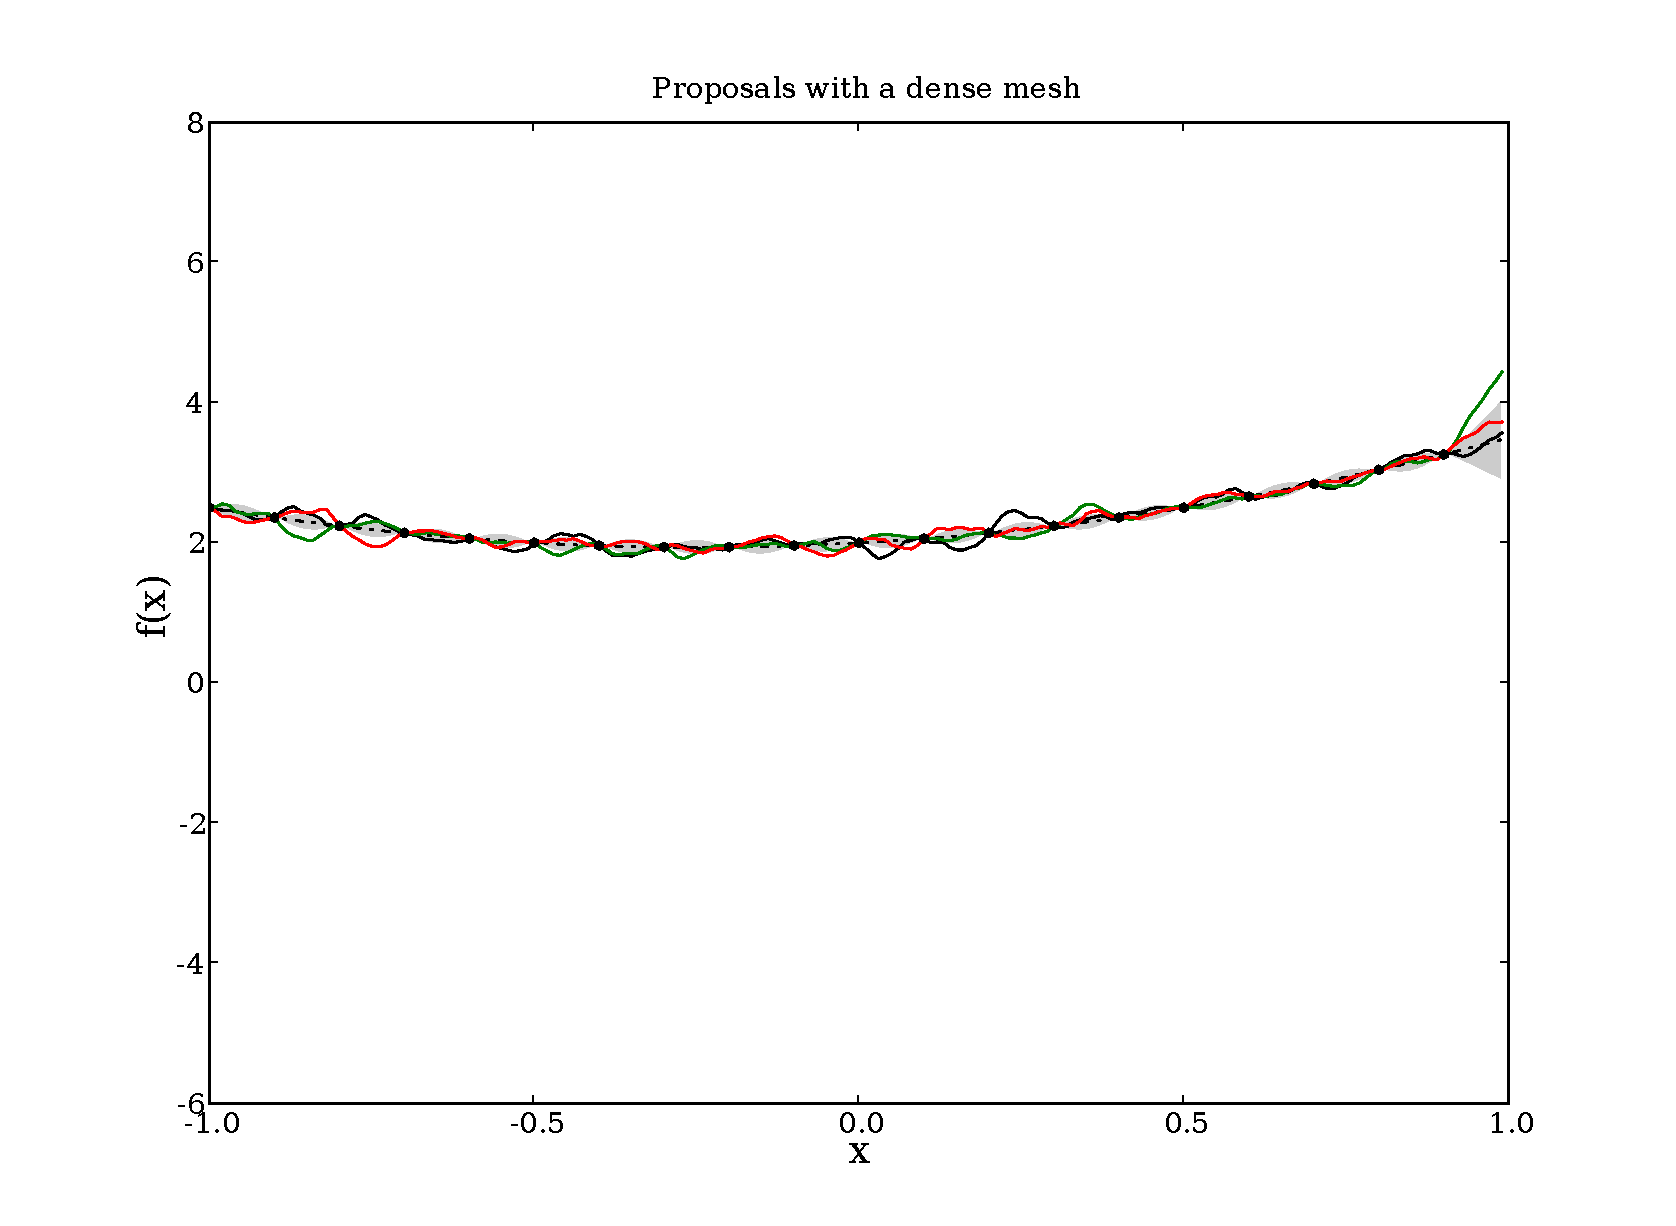
\epsfig{file=figs/densemeshpropose.pdf,width=5cm}
    \caption{Several possible proposals of $f$ (curves) given proposed values for $f(x_*)$ (heavy dots) with no mesh (left), a sparse mesh (middle), and a dense mesh (right). Proposal distributions'  $\pm$ one standard deviation envelopes are shown as shaded regions, with means shown as broken lines. With no mesh, $f$ is proposed from its prior and the acceptance rate will usually be very low. A denser mesh permits a high degree of control over $f$ and hence better acceptance ratios, but computing the log-probability is more expensive.}
    \label{fig:meshpropose}
\end{figure}


Figure~\ref{fig:meshchoice} provides a concrete example. To generate this figure, model~\ref{eq:simple-example-model} was created with meshes $x_*$ of varying densities, distributed evenly over the interval $[-1,1]$. Recall that that example had four observation locations $o$ evenly spaced between $-.8$ and $.8$. In general neither $x_*$ nor $o$ needs to be evenly spaced. 10000 steps of the default step method for $f(x_*)$ and $(f|f(x_*))$, \code{GPEvaluationMetropolis}, were timed. 

The time per jump is fairly constant for nonzero mesh sizes up to about 64, after which it increases cubically as is typical of GP computations. The rejection rate is close to 1 for mesh sizes up to about 16, after which it decreases. As illustrated in figure~\ref{fig:meshpropose}, large mesh spacings allow excessively large proposal jumps between mesh points, leading to high rejection rates. In this example, a happy medium is attained for mesh sizes in the neighborhood of 128. Of course, this will not be the case in all applications.

\begin{figure}
    \centering
        \epsfig{file=figs/meshchoice.pdf,width=15cm}
    \caption{The effects of mesh density on the performance of the Metropolis-Hastings jumping strategy described in section~\ref{sec:step-methods}. As mesh density increases, rejection rate tends to decrease, but the time required per jump increases. When the observation locations are known in advance, the mesh can be set to the observation locations for improved performance metrics marked by the two points. In this example, there are four observation locations, so the points are placed above the corresponding mesh size to provide a like-for-like comparison.}
    \label{fig:meshchoice}
\end{figure}

If $f$'s children depend on its value only via its evaluation on the mesh, that is if $x_*$ coincides with the observation locations, then the likelihood terms $p(K|f_p)$ and $p(K|f)$ will cancel. In other words, if the mesh is chosen so that $p(K|f)=p(K|f(x_*))$ then the proposed value of $f$ will have no bearing on the acceptance probability of the proposed value of $f(x_*)$ or of the parents $P$. The dots in figure~\ref{fig:meshchoice} show the rejection rate and time per jump for a modified version of model~\ref{eq:simple-example-model}, in which $o$ is known a priori and $x_*=0$. 

Both performance measures compare favorably to all of the mesh trials. Because the datapoints fall on mesh points, the uncontrolled proposal variance between mesh points illustrated in figure~\ref{fig:meshpropose} does not inflate rejection rates. Because the GP $f$ only needs to be evaluated at the four points $x_*=o$ throughout all of the jumps, the amount of computation needed is less than it is in any mesh trial except the length-0 trial and the time required per jump is also relatively low.

\subsection{Gibbs steps} 
\label{sec:gp-gibbs} 
If all of $f$'s children, $K$, depend on it as follows:
\begin{equation}
    \label{eq:gibbs-criterion} 
    K_i|f \stackrel{\textup{\tiny ind}}{\sim} \textup{Normal}(f(x_{*i}),V_i)
\end{equation}
then the full conditional distribution of both $f$ and $f(x_*)$ is of a standard form and both can be handled by the \code{GPEvaluationGibbs} step method. This step method is used in \code{MCMC.py}:
\begin{CodeChunk}
\begin{CodeInput}
GPSampler.use_step_method(gp.GPEvaluationGibbs, GPSampler.sm, \
    GPSampler.V, GPSampler.d)
\end{CodeInput}
\end{CodeChunk}
The initialization arguments are the GP submodel that contains $f$, the observation variance of $f$'s children, and the children, in this case the vector-valued normal variable $d$. 

\code{GPEvaluationGibbs} covers the standard submodel encountered in geostatistics, but there are many conjugate situations to which it does not apply. If necessary, special step methods can be written to handle these situations. If \code{GPEvaluationGibbs} is not assigned manually, $f(x_*)$ will be handled by the default \code{GPEvaluationMetropolis} step method, which will provide inferior performance. 


\section{Example: Duffy negativity prevalence in Africa}
\label{sec:duffy} 

\cite{Howes} recently presented global maps of the prevalence of Duffy negativity, a genetic trait in humans that confers resistance to infection by the malaria parasite \emph{Plasmodium vivax} \citep{duffy-vivax}. The geostatistical analysis that produced the maps was implemented using this package, and demonstrates its ability to support a model space that extends outside the standard generalized linear model family. 

The original implementation is freely available on the internet \citep{duffy-code, generic-mbg}. Code implementing a simplified version of the same analysis is included in the folder \\\code{pymc/examples/gp/more_examples/Duffy}. The current section will focus on this simplified version. Files \code{model.py} and \code{mcmc.py} contain the model specification and the model-fitting and predictive simulation procedure, respectively. The datafile \code{duffy-jittered.csv} contains a simulated dataset designed to produce a similar posterior distribution to the dataset collected by \cite{Howes} in Africa and the Arabian peninsula. 

\subsection{Scientific background and data}
\label{subsec:duffy-data} 
The Duffy negativity phenotype, as modelled by \cite{Howes}, is controlled by two genetic loci on chromosome 1. The first contains one of two alleles, known as \emph{FY*A} and \emph{FY*B}. These alleles encode proteins known as Fy$^\textup{a}$ and Fy$^\textup{b}$, respectively. The second locus can contain an allele that prevents expression of these proteins. A person is called `Duffy negative' if they do not express either protein Fy$^\textup{a}$ or Fy$^\textup{b}$, that is if each of their two copies of chromosome 1 contains the silencing allele. 

For clarity, in the remainder of this section the event that \emph{FY*A} is present at the first locus in a particular chromosome will be denoted $a$, and the event that \emph{FY*B} is present by $b$. Events $a$ and $b$ are, for the purposes of this model, mutually exclusive and all-inclusive. Similarly, the event that the silencing allele is present at the second locus will be denoted $s$. The genotype of said chromosome will be denoted by juxtaposing the events at the two loci: $as$, $b\neg s$, etc. The genotype of a person will be denoted as an unordered pair of chromosomal genotypes: $(bs,a \neg s)$, etc.

\cite{Howes} collected a comprehensive database of Duffy blood group surveys from the literature. In each survey, data collectors performed a test on a randomly-selected subset of a local population. They reported the test they used, number of individuals surveyed, the number classified into each output category of the chosen test, and the  The times, places, and motivations of the surveys, as well as the definitions of a `population', varied. The data and data abstraction protocol are described in detail by \cite{Howes}. 

Each survey in the database applied one of the following five tests to each participant:
\begin{description}
    \item[genotypic] This test determined participants' genotypes, and
could distinguish all ten possible genotypes $(bs,bs)$, $(as,bs)$, $(b\neg s,bs)$, \ldots
    \item[promoter] This test also examined participants' DNA directly, but only determined whether the silencing variant was present in either or both of each participant's copies of chromosome 1.
    \item[phenotypic] This test assayed participants' blood for proteins Fy$^\textup{a}$ and Fy$^\textup{b}$, rather than examining their genotypes directly.
    \item[a-phenotypic] This test also assayed participants' blood for proteins, but only determined whether Fy$^\textup{a}$ was expressed.
    \item[b-phenotypic] These studies only determined whether participants expressed Fy$^\textup{b}$.
\end{description}
The respective abilities of the tests to distinguish between the ten possible genotypes are illustrated in table \ref{tab:surveys}.

\begin{table}
    \centering
    \begin{small}
        \begin{tabular}{ccccccccccc}
            &$bs,bs$&$bs,as$&$as,as$&$b\neg s,b\neg s$&$b\neg s,a\neg s$&$a\neg s,a\neg s$&$bs,a\neg s$&$b\neg s,as$&$bs,b\neg s$&$as,a\neg s$\\
            \hline\hline
            genotypic&1&2&3&4&5&6&7&8&9&10\\
            promoter&1&1&1&2&2&2&2&2&2&2\\
            phenotypic&1&1&1&2&3&4&4&2&2&4\\
            a-phenotypic&1&1&1&1&2&2&2&1&1&2\\
            b-phenotypic&1&1&1&2&2&1&1&2&2&1
            \label{tab:equiv-class}
        \end{tabular}            
    \end{small}
    \caption{The ability of the five tests used by data collectors in the Duffy negativity example to distinguish between the ten possible genotypes. A survey type is able to distinguish between genotypes if the numbers in the corresponding columns are different.}
    \label{tab:surveys}  
\end{table}

\subsection{Statistical model}
The prevalence of Duffy negativity can be computed directly from \textbf{genotypic}, \textbf{promoter} and \textbf{phenotypic} surveys. If the entire dataset consisted of such observations the standard spatial generalized linear model framework could be applied \citep{diggle}. The other datatypes are not direct observations of the quantity to be predicted, but they are closely related and can be expected to contain valuable information that should be incorporated in the statistical analysis.

However, incorporating all of these datatypes in a geostatistical analysis requires a departure from the generalized linear model family. A simplified version of the model for these fields chosen by \cite{Howes}, and implemented in \code{model.py}, is given below. 

The targets of the inference are $p(b;x)$, the probability that event $b$ occurs in a randomly-chosen copy of chromosome 1 from location $x$; $p(s;x|b)$, the probability that event $s$ occurs in a randomly-chosen copy of chromosome 1 from location $x$ given than event $b$ occurs in the same chromosome; and $p(s;x|a)$, the probability that event $s$ occurs in a randomly-chosen copy of chromosome 1 from location $x$ given that event $a$ occurs in the same chromosome. The first two, $p(b;x)$ and $p(s;x|b)$, are modelled as functions from the Earth's surface to the interval $[0,1]$. Priors for these surfaces are constructed by transforming GP's, as described below. The last, $p(s;x|a)$, is modelled as a simple unknown constant $p_1$ because $s$ is rarely found in conjunction with $a$.

Two construct priors for the two unknown surfaces, the model declares two GPs, denoted $f_b$ and $f_s$. `Noisy' versions $\tilde f_b$ and $\tilde f_s$ are generated by adding an iid normal random variate at each location $x$ on the surface of the earth. The variances of these noisy versions are labelled $V_b$ and $V_s$, respectively. A nonlinear inverse logit transformation of $\tilde f_b$ generates $p(b;x)$, and likewise for $\tilde f_s$ and $p(s;x|b)$.

The covariances of the GPs $f_s$ and $f_b$ are are of the exponential form, with distance $d(x,y)$ between locations $x$ and $y$ defined as great-circle distance. This covariance function is positive definite \citep{spherical-validity}. The amplitude parameters are denoted $\phi_s$ and $\phi_b$, respectively, and the scale parameters are denoted $\theta_s$ and $\theta_b$. The mean of $f_s$ is modelled as zero. The mean of $f_b$ is modelled as $\beta\ 1(x\in r)$, where $\beta$ is an unknown scalar coefficient, $1(\cdot)$ is the indicator function and $r$ is the region south of the Sahara. \cite{Howes} chose this covariate because the prevalence of $b$ is known to decline sharply north of the Sahara.

The form of the prior $Q$ for the unknown scalar parameters $\phi_b$, $\theta_b$, $\phi_s$, $\theta_s$, $p_1$, $V_b$, $V_s$, $\beta$ does not affect the subsequent discussion, and is suppressed for brevity. The prior is, of course, written out in code in \code{model.py}. As in most Bayesian analyses, all of the unknown parameters are inferred along with the actual targets. 

In Bayesian hierarchical notation, the model as described so far is as follows:
\begin{equation}
    \label{eq:duffy-model} 
    \begin{array}{r}
        \phi_b,\theta_b,\phi_s,\theta_s,p_1,V_b,V_s\beta\sim Q\\
        C_{\phi,\theta}(x,y)=\phi\exp\left[{-\frac{d(x,y)}{\theta}}\right]\\\\
        M_b(x) = \beta\ 1(x\in r)\\
        f_b|\phi_b,\theta_b,\beta\sim \textup{GP}(M_b, C_{\phi_b,\theta_b}) \\
        \tilde f_b(x) | f_b(x) \stackrel{\textup{\tiny ind}}{\sim} \textup{N}(f_b(x),V_b) \\\\
        M_s(x) = 0\\
        f_s|\phi_s,\theta_s\sim \textup{GP}(M_s, C_{\phi_s,\theta_s})\\
        \tilde f_s(x) | f_s(x) \stackrel{\textup{\tiny ind}}{\sim} \textup{N}(f_s(x),V_s)\\\\
        p(b;x) = \textup{logit}^{-1}(\tilde f_b(x))\\
        p(s;x|b)= \textup{logit}^{-1}(\tilde f_s(x))\\
        p(s;x|a)= p_1
    \end{array}
\end{equation}  

The model is completed by likelihoods that give the probability of each survey outcome given the values of $p(b;o)$, $p(s;o|b)$ and $p(s;o|a)$ at the corresponding survey locations $o$. These likelihoods are described in detail by \cite{Howes}. Briefly, the promoter, a-phenotypic, and b-phenotypic tests all classify each survey participant into one of two categories, so the likelihoods corresponding to surveys that used these tests are binomial. The genotypic and phenotypic tests classify each survey participant into one of several categories, so the likelihoods corresponding to surveys that used them are multinomial. \cite{Howes} modelled the actual classification probabilities as functions of $p(b;o)$, $p(s;o|b)$ and $p(s;o|a)$ using the Hardy-Weinberg model from population genetics \citep{gillespie}, which assumes that an individual's two copies of an allele are chosen independently from a gene pool. 
The likelihoods are implemented in \code{model.py} using \pkg{PyMC}'s \code{Binomial} and \code{Multinomial} classes.

\subsection{Model fitting and prediction}
The portion of \code{mcmc.py} that creates the model and runs the sampling loop is quite concise: 
\begin{CodeInput}
DuffySampler = pymc.MCMC(model.make_model(**data), db='hdf5', dbcomplevel=1, \
    dbcomplib='zlib', dbname='duffydb.hdf5')

DuffySampler.use_step_method(pymc.gp.GPEvaluationGibbs, DuffySampler.sp_sub_b, \
    DuffySampler.V_b, DuffySampler.tilde_fb)

DuffySampler.use_step_method(pymc.gp.GPEvaluationGibbs, DuffySampler.sp_sub_s, \
    DuffySampler.V_s, DuffySampler.tilde_fs)

DuffySampler.isample(50000,10000,100)    
\end{CodeInput}
The first line creates the variables specified in \code{model.py}, and hands them to an MCMC sampler called \code{DuffySampler}. The database backend chosen is \code{hdf5}, so dynamic traces will be stored in an on-disk \pkg{PyTables} database under compression \citep{pymc}. The middle two lines choose the \code{GPEvaluationGibbs} step method, described in Section~\ref{sec:gp-gibbs}, for updating the \code{Gaussian process}es. This jumping strategy is applicable because the observation locations $o$ are known in advance, and because dependence of the children $\tilde f_b(o)$ of $f(o)$ is of the special form~\ref{eq:gibbs-criterion}, and likewise for $\tilde f_s$ and $f_s$. The final line calls for 50k MCMC iterations, with every 100 iterations after the first 10k saved to the database. 

While the sampler is running, a special prompt is displayed in the terminal window:
\begin{tiny}
    \begin{CodeInput}
        ==============
         PyMC console
        ==============

                PyMC is now sampling. Use the following commands to query or pause the sampler.


                Commands:
                  i -- index: print current iteration index
                  p -- pause: interrupt sampling and return to the main console.
                              Sampling can be resumed later with icontinue().
                  h -- halt:  stop sampling and truncate trace. Sampling cannot be
                              resumed for this chain.
                  b -- bg:    return to the main console. The sampling will still
                              run in a background thread. There is a possibility of
                              malfunction if you interfere with the Sampler's
                              state or the database during sampling. Use this at your
                              own risk.

        pymc > Sampling:   0% [                                                ] Iterations: 0
    \end{CodeInput}    
\end{tiny}
Sampling can be paused and resumed, or halted altogether, at any time. As sampling iterations are completed, the status bar fills up. When sampling is complete, control returns to the ordinary Python prompt. At this point, MCMC traces can be retrieved from \code{DuffySampler}. \code{DuffySampler.trace('p_1')[:]} returns the recorded samples of unknown scalar variable $p_1$ as a NumPy array and \code{DuffySampler.trace('sp_sub_b_f_eval')[:]} returns recorded samples of vector-valued variable $f_b(o)$. If desired, these traces can easily be plotted, subjected to convergence diagnostics or checked for autocorrelation. \code{DuffySampler.trace('sp_sub_b_f')[:]} returns recorded samples of the \code{Realization}-valued GP $f_b$. Each element in this trace matches the corresponding element of the trace at $f_b(o)$ at the observation locatinos $o$.

\bigskip
Most of the code in \code{mcmc.py} is devoted to estimating the mean and standard deviation of the posterior predictive distribution of Duffy negativity prevalence at unsampled locations $x$ in Africa and the Arabian peninsula (Figure~\ref{fig:duffymaps}). For each sample from the joint posterior of the variables in model~\ref{eq:duffy-model}, 
the pointwise mean and variance 
\begin{equation}
    \label{eq:map-moments} 
    \begin{array}{l}
        \E(f_b(x_i)|f_b(o), \phi_b, \theta_b, \beta)\\
        \VAR(f_b(x_i)|f_b(o), \phi_b, \theta_b, \beta)\\\\
        \E(f_s(x_i)|f_s(o), \phi_s, \theta_s)\\
        \VAR(f_s(x_i)|f_s(o), \phi_s, \theta_s)
    \end{array}
\end{equation}
are computed for each pixel $x_i$ in the output map. Using these moments, joint samples for $\tilde f_b(x_i)$ and $\tilde f_s(x_i)$ are obtained for each element $x_i$ of $x$. The last three lines of model~\ref{eq:duffy-model} are used to convert these to posterior predictive samples of the prevalence of the silencing variant, $p(s;x_i)$, and thence the prevalence of the Duffy negativite phenotype, $p(s;x_i)^2$. The posterior predictive mean and standard deviation of Duffy negativity prevalence are estimated from these samples, and these quantities are displayed on a map.

\bigskip
The algorithm just described is implemented simply and conveniently in \code{mcmc.py} using the \code{remember} method of \pkg{PyMC}'s \code{MCMC} objects, and the \code{point_eval} function provided by this package. The \code{remember} method of \code{DuffySampler} is used to reset its constituent variables to each of the $n$ stored samples from the joint posterior distribution:
\begin{CodeInput}
for i in xrange(n):
    DuffySampler.remember(0,i)
\end{CodeInput}
Inside the loop, the pointwise means and variances of equation~\ref{eq:map-moments} are computed efficiently and in a multithreaded fashion (on multi-core systems, assuming the environment variable \code{OMP_NUM_THREADS} is set to a value greater than 1) using \code{point_eval}:
\begin{CodeInput}
    Msurf_b, Vsurf_b = pymc.gp.point_eval(DuffySampler.sp_sub_b.M_obs.value, \
        DuffySampler.sp_sub_b.C_obs.value, dpred)
    
    Msurf_s, Vsurf_s = pymc.gp.point_eval(DuffySampler.sp_sub_s.M_obs.value, \
        DuffySampler.sp_sub_s.C_obs.value, dpred)
\end{CodeInput}
The `nugget' variances $V_b$ and $V_s$ are added to the variances in equation~\ref{eq:map-moments} to obtain the conditional variances of $\tilde f_s$ and $\tilde f_b$:        
\begin{CodeInput} 
    Vsurf_b += DuffySampler.V_b.value
    Vsurf_s += DuffySampler.V_s.value
\end{CodeInput}
 Samples from these distributions are drawn, and converted to posterior predictive samples for the frequencies $p(s|b;x_i)$ and $p(b;x_i)$ at each pixel $x_i$:
\begin{CodeInput}
    freq_b = pymc.invlogit(Msurf_b + pymc.rnormal(0,1)*np.sqrt(Vsurf_b))
    freq_s = pymc.invlogit(Msurf_s + pymc.rnormal(0,1)*np.sqrt(Vsurf_s))
\end{CodeInput}
Finally, these samples are converted to a posterior predictive sample for Duffy negativity prevalence $p(s;x_i)^2=[p(s;x_i|b)p(b;x_i)+p(s;x_i|a)p(a;x_i)]^2$:
\begin{CodeInput}
    samp_i = (freq_b*freq_s+(1-freq_b)*DuffySampler.p1.value)**2
\end{CodeInput}
These samples are accumulated to produce estimates of the first two moments of the posterior predictive distribution of $p(s;x_i)^2$ for each $x_i$, and these moments are used to fill in the maps of the posterior predictive mean and standard deviation shown in Figure~\ref{fig:duffymaps}.

\begin{figure}
\begin{center}
    \epsfig{file=figs/duffymean.pdf, width=7cm} 
    \epsfig{file=figs/duffyvar.pdf, width=7cm}     
    \caption{The mean and variance of the posterior predictive distribution of Duffy negativity prevalence, $p(s;x)^2$ in the notation of model~\ref{eq:duffy-model}, in Africa and the Arabian peninsula. These maps were produced by \code{pymc/examples/gp/more_examples/Duffy/mcmc.py}. The locations of (simulated) observations are shown as red dots. In general, the data support low prevalences in northern and southern Africa, and higher prevalences in central Africa. Predictive variance is low in the neighborhoods of survey locations and where the data indicate that prevalence is either very high or very low. The discontinuity at the boundary between the Sahara and the Sahel delimits the region $r$, which is used to generate the linear covariate $1(x\in r)$. Because the mapped quantity is a nonlinear function of the GP $f_b$, its variance is affected by shifts in the mean of $f_b$. }
    \label{fig:duffymaps}
\end{center}    
\end{figure}

% \begin{figure}
%     \centering
%         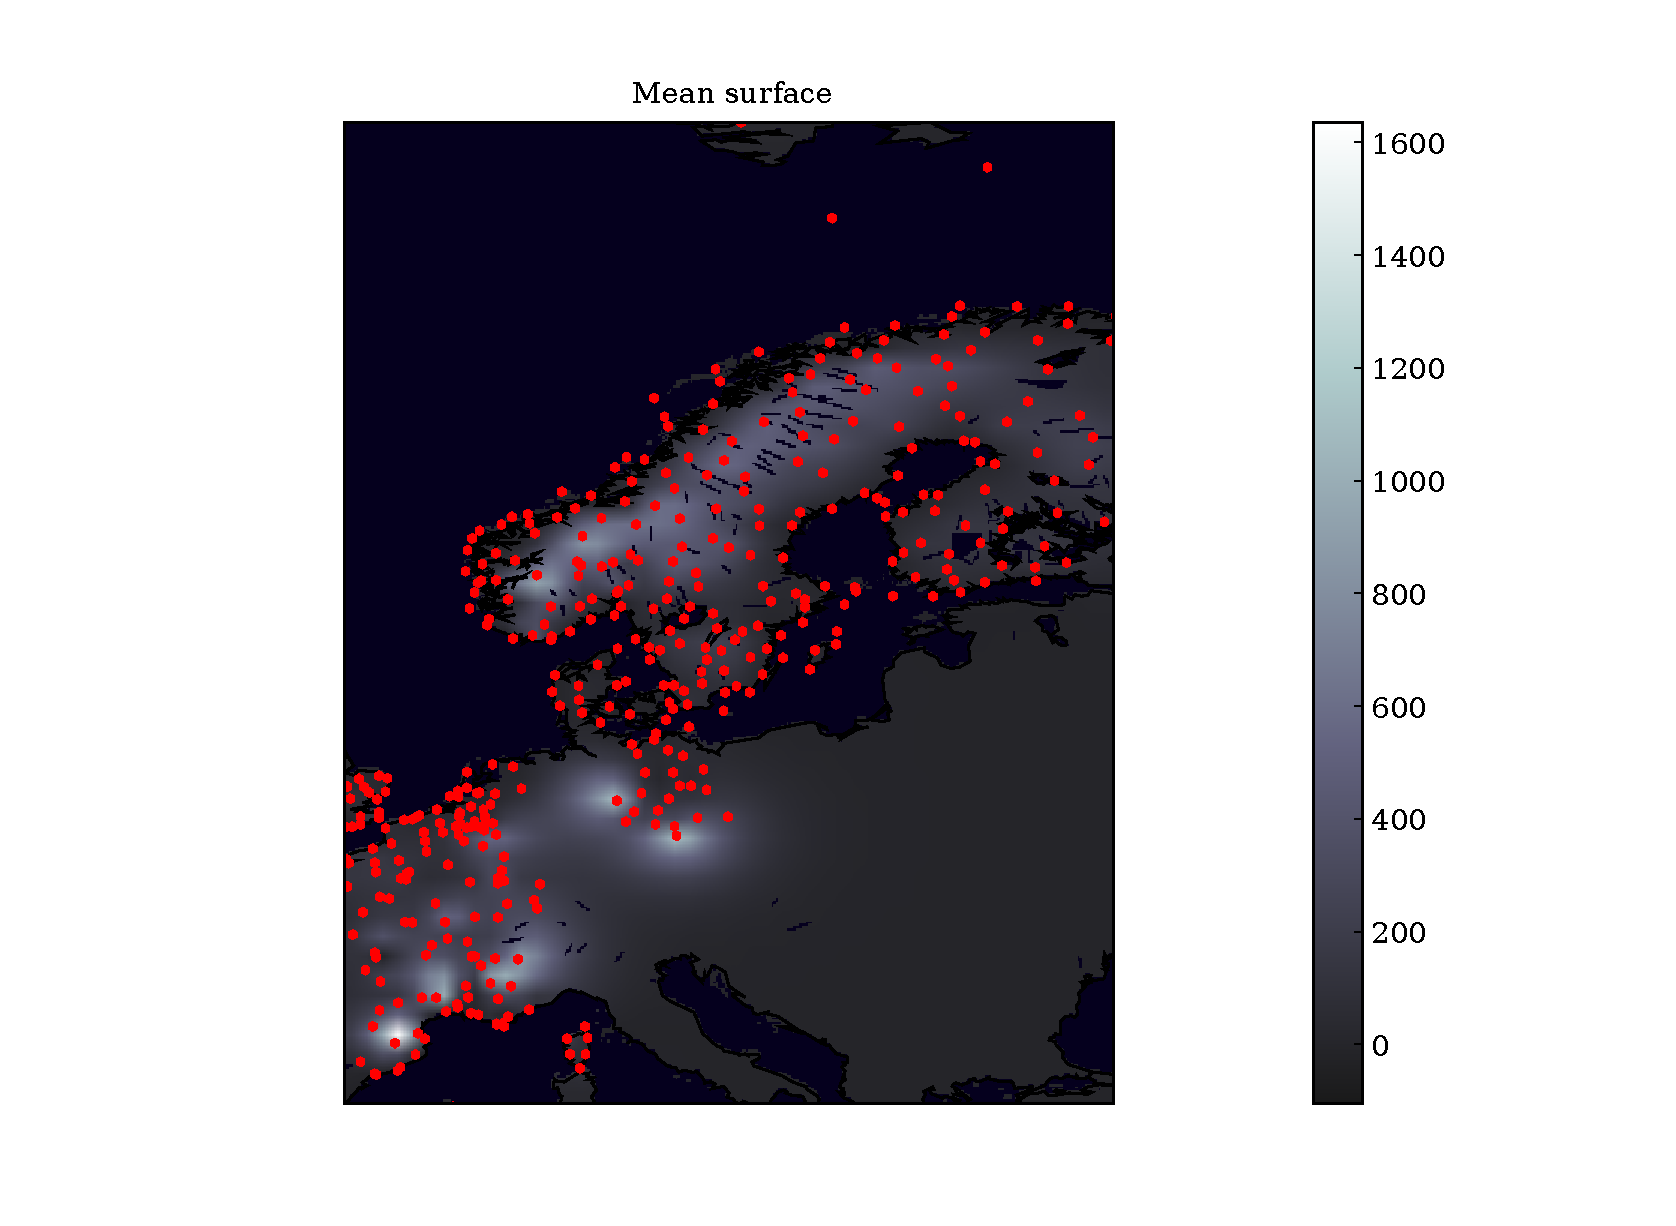
\epsfig{file=figs/elevmean.pdf, width=7cm}
%         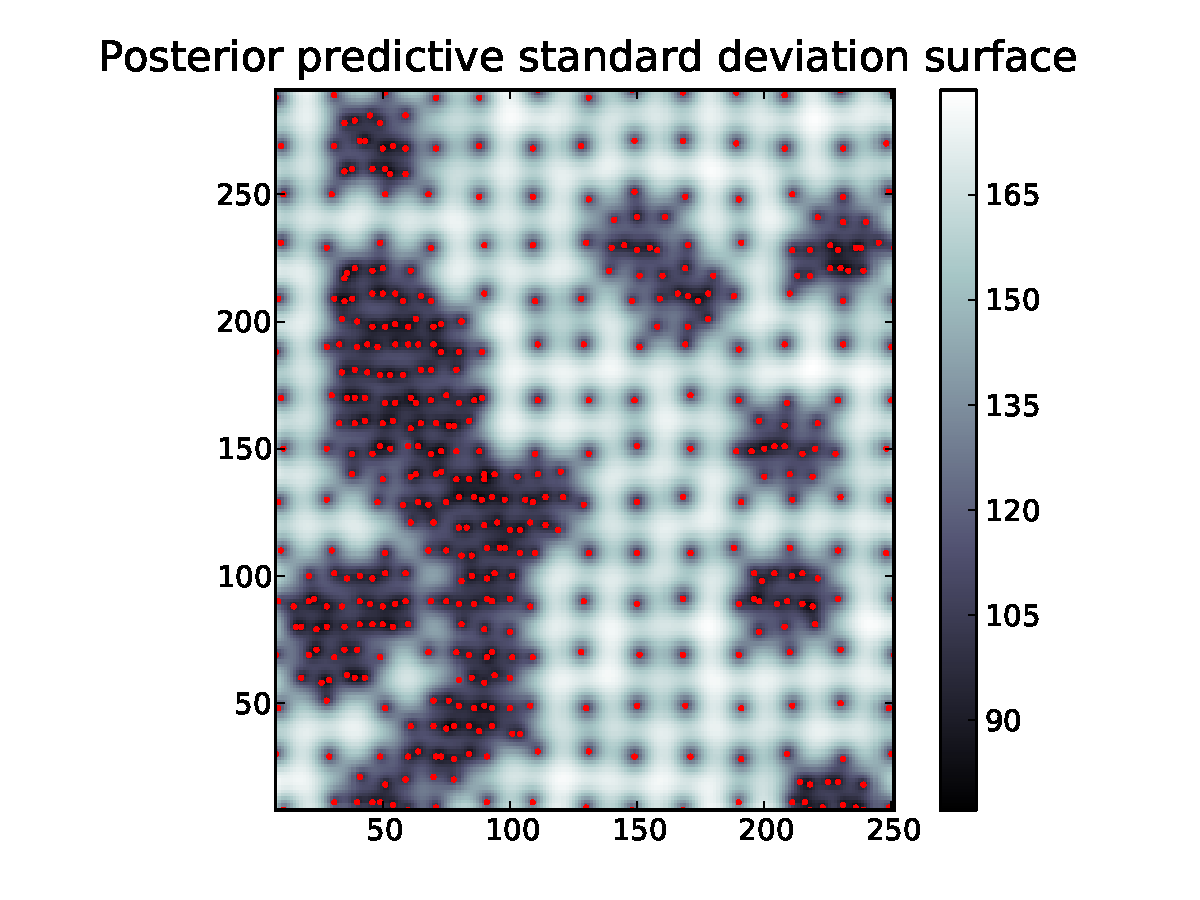
\epsfig{file=figs/elevvar.pdf, width=7cm}
%     \caption{The posterior mean and variance surfaces for the $v$ variable of the Walker lake example. The posterior variance is relatively small in the neighborhood of observations, but large in regions where no observations were made.}
%     \label{fig:walker}
% \end{figure}
% \begin{figure}
%     \centering
%         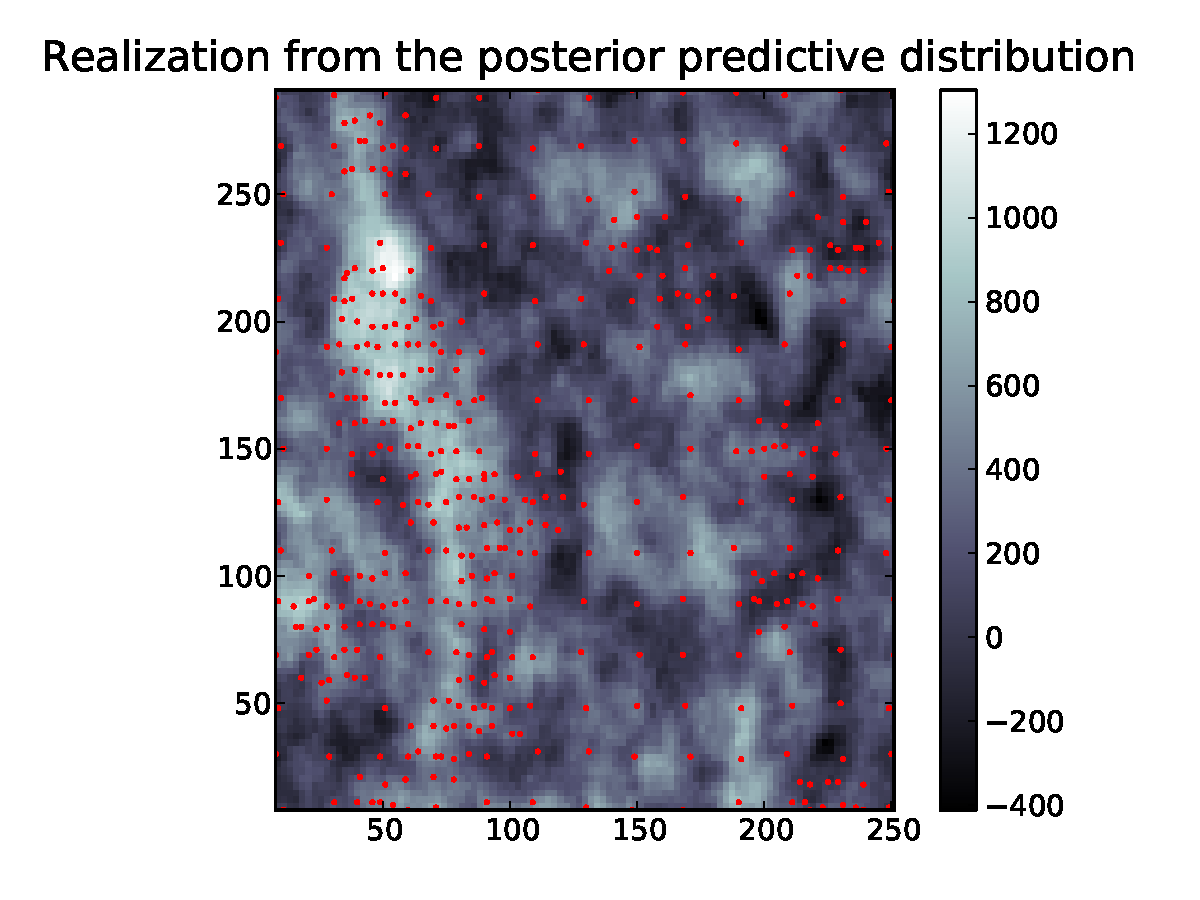
\epsfig{file=figs/elevdraw0.pdf, width=7cm}
%         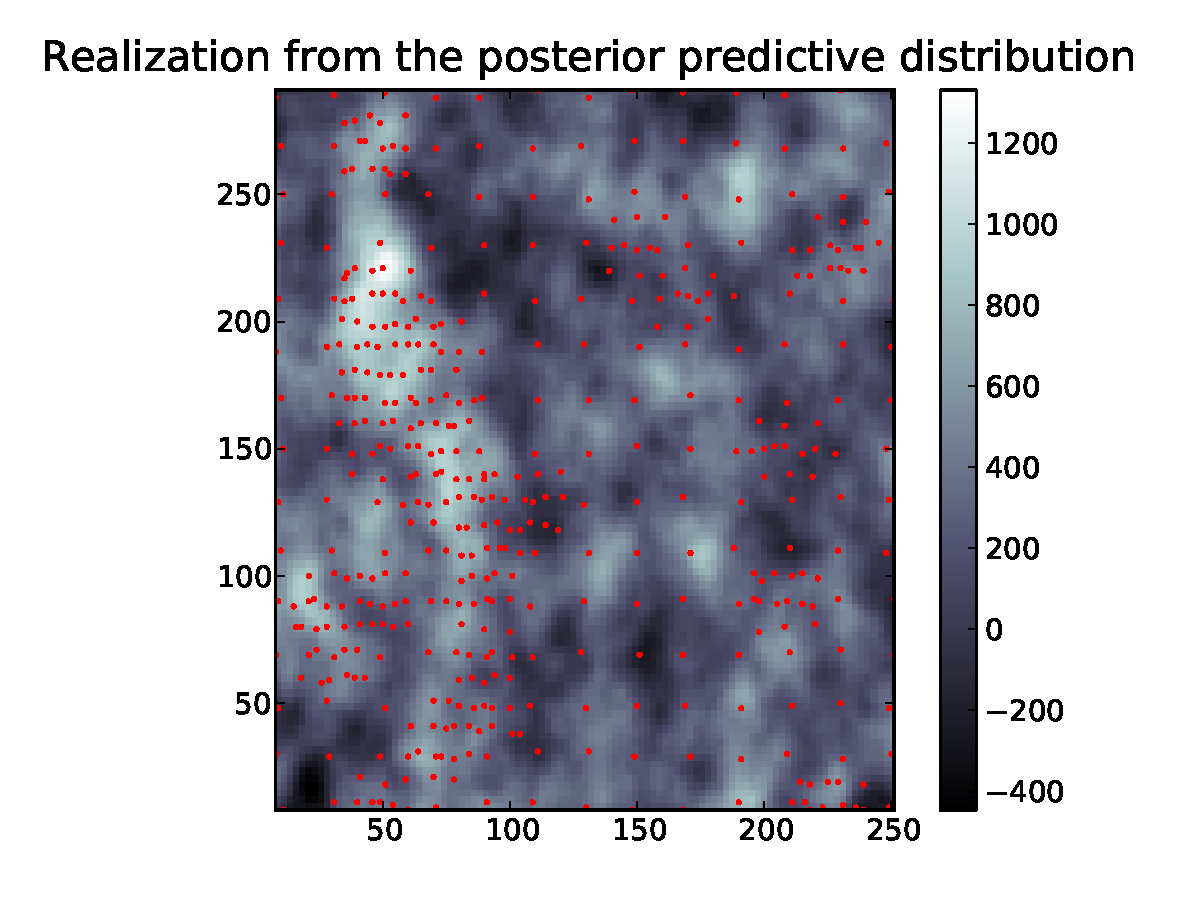
\epsfig{file=figs/elevdraw1.pdf, width=7cm}
%     \caption{Two realizations from the posterior distribution of the $v$ surface for the Walker Lake example. Elevation is measured in meters.}
%     \label{fig:walkerreal}
% \end{figure}
% Bayesian geostatistics is demonstrated in the folder \code{pymc/examples/gp/more_examples/Geostatistics}. File \code{getdata.py} downloads the Walker Lake dataset of Isaaks and Srivastava \citep{isaaks} from the internet and manipulates the $x$ and $y$ coordinates into the array format described in section \ref{sec:highdim}. File \code{model.py} contains the geostatistical model specification, which is
% 
% \begin{eqnarray*}
%     d|f \sim \textup{Normal}(f(x),V)\\
%     f|M,C \sim \textup{GP}(M,C) \\
%     M:x\rightarrow m\\
%     C:x,y,\mathtt{amp},\mathtt{scale},\mathtt{diff\_degree}\rightarrow \mathtt{matern.euclidean}(x,y;\mathtt{amp},\mathtt{scale},\mathtt{diff\_degree})\\
%     p(m)\propto 1\\
%     \mathtt{amp}\sim \textup{Exponential}(7e-5) \\
%     \mathtt{scale}\sim \textup{Exponential}(4e-3) \\
%     \mathtt{diff\_degree}\sim \textup{Uniform}(.5,2)\\ 
%     V\sim \textup{Exponential}(5e-9)\\
% \end{eqnarray*}
% 
% File \code{mcmc.py} fits the model and produces output maps.  The output of \code{mcmc.py} is shown in figures \ref{fig:walker} and \ref{fig:walkerreal}. Figure \ref{fig:walker} shows the posterior mean and variance of the $v$ variable of the dataset, which is a function of elevation (see \cite{isaaks}, appendix A).

\section{Conclusion}

This package is built around the \code{Realization} object, which represents random mathematical functions as random \proglang{Python} functions. This is arguably the most natural and intuitive representation possible within the \proglang{Python} programming language, which itself is widely regarded as unusually human-friendly. 

This design choice has concrete advantages that go beyond aesthetics. The Duffy negativity example in Section~\ref{sec:duffy} implements a probability model (model~\ref{eq:duffy-model}) that is not a member of the spatial generalized linear model family, whose nonstandard likelihood function involves transformations of two GPs. It would not be possible to implement in a model-based geostatistics package that specializes to spatial generalized linear models. However, this package focuses on providing a \pkg{Python} representation of GPs that closely resembles the mathematical objects rather than on covering any particular model family. Because model~\ref{eq:duffy-model} is straightforward to express in terms of those mathematical objects, it falls comfortably within this package's scope. The highly declarative implementation in \code{pymc/examples/gp/more_examples/Duffy/model.py} is little more than a transliteration from mathematical notation to \pkg{Python}. 

This package inherits the flexibility of \pkg{PyMC}, as described in Section~\ref{sec:gp-sub}. Because \pkg{PyMC} allows any \proglang{Python} function to be used to transform variables in probability models, and \proglang{Python} (like all modern programming languages) allows functions to be passed to other functions as arguments, and \code{GaussianProcess} objects are function-valued random variables, this package supports construction of a very wide variety of probability models that involve scalar-valued GPs. In keeping with the extensible spirit of \pkg{PyMC}, this package accomodates user-specified mean and covariance functions, and provides support for automatic combination of covariance functions and distance metrics.

Strenuous efforts at optimization have resulted in good performance for `standard' GP-based analyses such as Bayesian geostatistics. For example, \cite{map} recently used it to conduct a fully Bayesian analysis involving a very expensive covariance function evaluated at 4,291 input locations. The library of covariance functions provided by the package is implemented in Fortran, and can take advantage of SMP systems. The linear algebra functionality is provided by \pkg{NumPy}, which can be configured to make use of optimized, multithreaded \pkg{BLAS} \citep{blas} and \pkg{LAPACK} \citep{lapack}  implementations. 

However, there are many use cases for which this package cannot achieve performance on par with hand-optimized algorithms. For example, in many reversible-jump MCMC applications (e.g. \cite{gramacy}) the set of input locations under consideration changes as the MCMC progresses. It would be possible to create these models and start to fit them using this package, but the acceptance rate would typically be much lower than that enjoyed by a true reversible-jump MCMC algorithm for reasons explained in Section~\ref{sec:step-methods}. It remains to be seen whether this and related performance problems can be overcome without either diluting the conceptual fidelity of the object model or incurring an unmanageable amount of additional complexity.

More tutorial material, as well as documentation of several additional features and the incomplete Cholesky decomposition algorithms, can be found in the full package documentation at \href{http://pymc.googlecode.com/files/GPUserGuide.pdf}{http://pymc.googlecode.com/files/GPUserGuide.pdf}.

% \nocite{*}
% \bibliographystyle{plain}v
\bibliography{jss-gp}

\end{document}
